\chapter[Données et objets]{Données et objets}
\label{chap:VIII}

\lettrine{L}{e \href{https://eduscol.education.fr/cid143713/snt-bac-2021.html}{programme officiel SNT} définit sept champs d'investigation}. Les \linebreak quatre premiers abordés dans ce chapitre concernent les données et les objets connectés, à savoir : les données structurées et leur traitement, la photographie numérique, l'informatique embarquée et les objets connectés, la localisation et la cartographie. 

Chaque thématique possède un canevas commun : « Découvrir la thématique » et « Réaliser des activités ». Si la première de ces sections vise la présentation du sujet, la seconde est ouverte aux suggestions et amenée à intégrer les contributions des enseignants. 

Il va sans dire que chaque thème énoncé bénéficie des contenus exposés dans les autres parties du document, notamment \qnameref{part:I} et \qnameref{part:II}.

%----------
\section[Données et traitements]{Données et traitements}
\label{sec:.VIII.1}


\subsection[Découvrir la thématique]{Découvrir la thématique}
\label{sub:VIII.1.1}

\subsubsection[Ancrage dans le réel]{Ancrage dans le réel}
\label{subsub:VIII.1.1.1}

\overparagraph{Points-clés}

\begin{jazzitemize}
\item L'information humaine est transcrite sous forme de données afin d'ê\-tre manipulée numériquement.
\item On distingue les données qui doivent être entrées dans la machine, des résultats de calculs, ou sortie des algorithmes. 
\item Les données en tant qu'objets numériques forment un bien non rival\parnote{\href{https://fr.wikipedia.org/wiki/Rivalit\%C3\%A9_(\%C3\%A9conomie)}{Bien non rival} : la plupart des objets matériels sont des biens rivaux c'est-à-dire que si on les consomme ou les utilise, ils ne sont plus disponibles pour les autres consommateurs,  ce n'est pas le cas des objets informationnels comme par exemple une bonne histoire : si je la partage, elle reste intacte, voire elle s'enrichit.}  dont la copie ne coûte quasiment rien, et que l'on peut dupliquer sans le consommer.
\item La production gigantesque de données pose des problèmes planétaires en matière d'environnement (consommation énergéti\-que, utilisation de ressources naturelles rares).
\item La prolifération de données pose également un problème de pérennité à long terme (à l'échelle de plusieurs dizaines d'années) non résolu actuellement.
\end{jazzitemize}
\parnotes

%\vfill\pagebreak

\overparagraph{Mots-clés}

\begin{marginvideo}
	[\label{vid:VIII.1}Données et traitements.]%
	%\movie[width=\marginparwidth,showcontrols]%
	%	{\includegraphics[width=\marginparwidth]{./Images/Pictograms/film-strip-dark-electric-blue.png}}%
	%	{./Videos/Chapter08/vidVIII-01-mooc-snt-data.mp4}%
	\href{https://www.youtube.com/watch?v=IJJgcZ2DEs0}%
	  {\includegraphics[width=\marginparwidth]{./Images/Pictograms/film-strip-dark-electric-blue.png}}%
	\launchvideo{https://www.youtube.com/watch?v=IJJgcZ2DEs0}
\end{marginvideo}

\begin{jazzitemize}
\item \href{https://fr.wikipedia.org/wiki/Big_data}{Mégadonnées} : (\textit{Big Data}) on parle de mégadonnée \nopagebreak quand le volume de données est tel qu'on peut faire des analyses statistiques qui permettent de prédire des informations, même si les données sont très diverses, sans information structurée, et approximatives.
\item \href{https://fr.wikipedia.org/wiki/Donn\%C3\%A9es_ouvertes}{Données ouvertes} : (Open Data)  données numériques, d'origine publique ou privée, diffusées de manière structurée selon une méthode et une licence libre, garantissant leur libre accès et leur réutilisation par toutes et tous, sans restriction technique, juridique ou financière.
\item \href{https://fr.wikipedia.org/wiki/Licence_libre}{Licence libre} : licence s'appliquant à une œuvre de l'esprit (document, logiciel, etc.) par laquelle l'autrice ou l'auteur concède les droits que lui confère le droit d'auteur  : usage de l'œuvre, étude de l'œuvre pour en comprendre le fonctionnement ou l'adapter à ses besoins, modification (amélioration, extension et transformation) ou incorporation de l'œuvre en une œuvre dérivée, redistribution de l'œuvre, c'est-à-dire sa diffusion à d'autres usagers, y compris commercialement.
\item \href{https://fr.wikipedia.org/wiki/Informatique_durable}{Informatique durable} : (green IT) vise à réduire l'empreinte écologique, économique et sociale des technologies de l'information et de la communication.
\item \href{https://fr.wikipedia.org/wiki/R\%C3\%A8glement_g\%C3\%A9n\%C3\%A9ral_sur_la_protection_des_donn\%C3\%A9es}{Règlement général sur la protection des données (RGPD)} :  renforce et unifie la protection des données pour les personnes au sein de l'Union Européenne.
\end{jazzitemize}

\overparagraph{Ce que dit le programme}

\begin{tcolorbox}[title={Introduction}, toprule=0pt, leftrule=0pt, rightrule=0pt, arc=0pt, fonttitle=\scshape\boxtitlefont,
                  colbacktitle=white, coltitle=firstcolor, colframe=firstcolor, colback=firstcolor!10,
                  breakable, enhanced jigsaw]
Les données constituent la matière première de toute activité numérique. Afin de permettre leur réutilisation, il est nécessaire de les conserver de manière persistante. Les structurer correctement garantit que l’on puisse les exploiter facilement pour produire de l’information. Cependant, les données non structurées peuvent aussi être exploitées, par exemple par les moteurs de recherche.
\end{tcolorbox}

\begin{tcolorbox}[title={Impacts sur les pratiques humaines}, toprule=0pt, leftrule=0pt, rightrule=0pt, arc=0pt,
                  fonttitle=\scshape\boxtitlefont,
                  colbacktitle=white, coltitle=firstcolor, colframe=firstcolor, colback=firstcolor!10,
                  breakable, enhanced jigsaw]
L’évolution des capacités de stockage, de traitement et de diffusion des données fait qu’on assiste aujourd’hui à un phénomène de surabondance des données et au développement de nouveaux algorithmes capables de les exploiter.

L’exploitation de données massives (\textit{Big Data}) est en plein essor dans des domaines aussi variés que les sciences, la santé ou encore l’économie. Les conséquences sociétales sont nombreuses tant en termes de démocratie, de surveillance de masse ou encore d’exploitation des données personnelles.

Certaines de ces données sont dites ouvertes (\textit{Open Data}), leurs producteurs considérant qu’il s’agit d’un bien commun. Mais on assiste aussi au développement d’un marché de la donnée où des entreprises collectent et revendent des données sans transparence pour les usagers. D’où l’importance d’un cadre juridique permettant de protéger les usagers, préoccupation à laquelle répond le règlement général sur la protection des données (RGPD).

Les centres de données (\textit{Data Center}) stockent des serveurs mettant à disposition les données et des applications les exploitant. Leur fonctionnement nécessite des ressources (en eau pour le refroidissement des machines, en électricité pour leur fonctionnement, en métaux rares pour leur fabrication) et génère de la pollution (manipulation de substances dangereuses lors de la fabrication, de la destruction ou du recyclage). De ce fait les usages numériques doivent être pensés de façon à limiter la transformation des écosystèmes (notamment le réchauffement climatique) et à protéger la santé humaine. 
\end{tcolorbox}

\subsubsection[Volet historique]{Volet historique}
\label{subsub:VIII.1.1.2}

\sidegraphic[Ada \textsc{Lovelace} (1815-1852).]{\includegraphics[width=\linewidth]{graphVIII-01-ada-lovelace.jpg}}%
L'idée de pouvoir traiter mécaniquement de l'information est ancienne, dès le XVII\frup{e} siècle, par exemple, Gottfried Wilhelm \textsc{Leibniz} va chercher à établir une langue dite caractéristique universelle, qui permettrait d'exprimer la totalité des pensées humaines et pourrait résoudre des problèmes par un calculateur (\textit{calculus ratiocinator}), anticipant l'informatique de plus de trois siècles. Il faudra attendre le XX\frup{e} siècle pour comprendre qu'une telle machine est un objet impossible ne serait-ce qu'en mathématiques, d'après les théorèmes d'Alonzo \textsc{Church} et Alan \textsc{Turing} : très simplement, certains calculs (par exemple savoir si un programme va boucler à l'infini, le problème de l'arrêt) nécessitent des temps... Infinis. On commençait à comprendre les limites de l'intelligence mécanique avant même de l'avoir fabriquée.

Ces mêmes personnes ont pourtant fondé, dans les années 1930, l'informatique, un domaine d'activité scientifique, technique et industriel concernant le traitement automatique de l'information par l'exécution de programmes informatiques par des machines. On peut attribuer à Ada \textsc{Lovelace}, un siècle avant, d'avoir compris que l'on peut «~calculer sur des nombres mais aussi sur des symboles », on parlerait de données numériques et symboliques aujourd'hui. Il est intéressant de noter que ces idées sont nées avant la technologie permettant de les mettre en œuvre.

\sidegraphic[John \textsc{von Neumann} (1903-1953).]{\includegraphics[width=\linewidth]{graphVIII-02-johnvonneumann-1940-wikipedia.jpg}}%
Parallèlement, dans les années 1880, Herman \textsc{Hollerith}, futur fondateur d'IBM, fonde la mécanographie en inventant une machine électromécanique destinée à faciliter le recensement en stockant les informations sur une carte perforée. Ces premières cartes perforées ont fait leur apparition au XVIII\frup{e} siècle dans divers automates et en particulier les métiers à tisser, les orgues de Barbarie et les pianos mécaniques.

L'histoire de l'informatique débute véritablement au milieu du XX\frup{e} siècle avec l'architecture de John \textsc{von Neumann}, mise en application dans la machine universelle d'Alan \textsc{Turing} : les ordinateurs dépassent la simple faculté de calculer et peuvent désormais commencer à traiter des données.

\overparagraph*{Ce que dit le programme}

\begin{tcolorbox}[title={Repères historiques}, toprule=0pt, leftrule=0pt, rightrule=0pt, arc=0pt,
                  fonttitle=\scshape\boxtitlefont,
                  colbacktitle=white, coltitle=firstcolor, colframe=firstcolor, colback=firstcolor!10,
                  breakable, enhanced jigsaw]
\begin{jazzitemize}
%\setlength{\itemsep}{1.5\parskip}
\item 1930 : utilisation des cartes perforées, premier support de stockage de  données.
\item 1956 : invention du disque dur permettant de stocker de plus grandes  quantités de données, avec un accès de plus en plus rapide.
\item 1970 : invention du modèle relationnel (E. L. \textsc{Codd}) pour la structuration et l’indexation des bases de données. 
\item 1979 : création du premier tableur, VisiCalc.
\item 2009 : \textit{Open Government Initiative} du président Obama.
\item 2013 : charte du G8 pour l’ouverture des données publiques.
\end{jazzitemize}
\end{tcolorbox}

\subsubsection[Explication des notions]{Explication des notions}
\label{subsub:VIII.1.1.3}

\overparagraph{Idées-forces}

\begin{jazzitemize}
\item Toutes les informations humaines se codent en binaire ; bien entendu ce n'est pas l'objet réel, ce n'est que son reflet numérique.
\item Une donnée est spécifiée par des valeurs et chaque valeur a un type (par exemple : vrai ou faux, on dit booléen ; ou bien numérique ou textuel ; ou encore un type spécifique, comme une date) ; selon le type de la donnée on ne fait pas les mêmes opérations.
\item Une donnée se décompose de manière atomique en données élémentaires, par exemple le nom d'une personne en prénom et patronyme. Bien structurer les données facilite leur traitement par des algorithmes.
\item Une collection de données peut être ordonnée sous forme de liste, ou bien sans ordre sous forme d'un ensemble.
\item La façon de structurer les données influe fortement sur les opérations de traitement : il est par exemple bien plus efficace de rechercher une donnée dans une collection toujours ordonnée, mais y insérer une information est plus coûteux.
\end{jazzitemize}

\overparagraph{Mots-clefs}

\begin{jazzitemize}
\item \href{https://fr.wikipedia.org/wiki/Donn\%C3\%A9e_(informatique)}{Donnée} : \href{https://fr.wikipedia.org/wiki/Repr\%C3\%A9sentation}{représentation} d'une \href{https://fr.wikipedia.org/wiki/Information}{information} au sein d'un système informatique.
\item \href{https://fr.wikipedia.org/wiki/M\%C3\%A9tadonn\%C3\%A9e}{Métadonnée} : \href{https://fr.wikipedia.org/wiki/Donn\%C3\%A9e_(informatique)}{donnée} servant à définir ou décrire une autre donnée, pour permettre sa manipulation.
\item Une \href{https://fr.wikipedia.org/wiki/Base_de_donn\%C3\%A9es}{base de données} regroupe plusieurs collections de données reliées entre elles.
\item \href{https://fr.wiktionary.org/wiki/descripteur}{Descripteur} : mot ou un groupe de mots choisi pour caractériser les informations contenues dans un document et pour faciliter les recherches.
\end{jazzitemize}

\overparagraph{Ce que dit le programme}

\begin{tcolorbox}[title={Données et information}, toprule=0pt, leftrule=0pt, rightrule=0pt, arc=0pt,
                  fonttitle=\scshape\boxtitlefont,
                  colbacktitle=white, coltitle=firstcolor, colframe=firstcolor, colback=firstcolor!10,
                  breakable, enhanced jigsaw]


Une \emph{donnée} est une valeur décrivant un objet, une personne, un événement digne d’intérêt pour celui qui choisit de la conserver. Le numéro de téléphone d’un contact est une donnée. Plusieurs \emph{descripteurs} peuvent être utiles pour décrire un même objet (par exemple des descripteurs permettant de caractériser un contact : nom, prénom, adresse et numéro de téléphone).

Une \emph{collection} regroupe des objets qui partagent les mêmes descripteurs (la collection des contacts d’un carnet d’adresses par exemple). La structure de table permet de présenter une collection : les objets en ligne, les descripteurs en colonne et les données à l’intersection. Les données sont alors dites structurées.

Pour assurer la persistance des données, ces dernières sont stockées dans des fichiers. Le format CSV (\textit{Comma Separated Values}, les données avec des séparateurs) est un format de fichier simple permettant d’enregistrer une table. À tout fichier sont associées des \emph{métadonnées} qui permettent d’en décrire le contenu. Ces métadonnées varient selon le type de fichier (date et coordonnées de géolocalisation d’une photographie, auteur et titre d’un fichier texte, etc.).

Les données comme les métadonnées peuvent être capturées et enregistrées par un dispositif matériel ou bien renseignées par un humain. Elles sont de différents types (numériques, textes, dates) et peuvent se traiter de manières diverses (calcul, tri, affichage, etc.).

Certaines collections typiques sont utilisées dans des applications et des formats standardisés leur sont associés : par exemple le format ouvert vCard (extension \texttt{.vfc}) pour une collection de contacts.

Une \emph{base de données} regroupe plusieurs collections de données reliées entre elles. Par exemple, la base de données d’une bibliothèque conserve les données sur les livres, les abonnés et les emprunts effectués.
\end{tcolorbox}


\begin{tcolorbox}[title={Algorithmes et programmes}, toprule=0pt, leftrule=0pt, rightrule=0pt, arc=0pt,
                  fonttitle=\scshape\boxtitlefont,
                  colbacktitle=white, coltitle=firstcolor, colframe=firstcolor, colback=firstcolor!10,
                  breakable, enhanced jigsaw]
La recherche dans des \emph{données structurées} a d’abord été effectuée selon une indexation préalable faite par l’homme. Des algorithmes ont ensuite permis d’automatiser l’indexation à partir de textes, d’images ou de sons.

Une table de données peut faire l’objet de différentes opérations : rechercher une information précise dans la collection, trier la collection sur une ou plusieurs propriétés, filtrer la collection selon un ou plusieurs tests sur les valeurs des descripteurs, effectuer des calculs, mettre en forme les informations produites pour une visualisation par les utilisateurs.

La recherche dans une base comportant plusieurs collections peut aussi croiser des collections différentes sur un descripteur commun ou comparable.
\end{tcolorbox}

\begin{tcolorbox}[title={}Machines, toprule=0pt, leftrule=0pt, rightrule=0pt, arc=0pt,
                  fonttitle=\scshape\boxtitlefont,
                  colbacktitle=white, coltitle=firstcolor, colframe=firstcolor, colback=firstcolor!10,
                  breakable, enhanced jigsaw]
Les fichiers de données sont stockés sur des supports de stockage : internes (disque dur ou SSD) ou externes (disque, clef USB), locaux ou distants (\textit{cloud}). Ces supports pouvant subir des dommages entraînant des altérations ou des destructions des données, il est nécessaire de réaliser des sauvegardes.

Des recherches dans les fichiers se font à l’intérieur même des ordinateurs, soit sur la base de leurs métadonnées, soit à partir d’une indexation (à la manière des moteurs de recherche disponibles sur le Web).

Les grandes bases de données sont souvent implémentées sur des serveurs dédiés (machines puissantes avec une importante capacité de stockage sur disques). Ces centres de données doivent être alimentés en électricité et maintenus à des températures suffisamment basses pour fonctionner correctement.
\end{tcolorbox}

\overparagraph{Web-conférence}

\begin{marginvideo}
	[\label{vid:VIII.2}Données structurées et traitements, Élisa \textsc{Fromont}.]%
	%\movie[width=\marginparwidth,showcontrols]%
	%	{\includegraphics[width=\marginparwidth]{./Images/Pictograms/film-strip-dark-electric-blue.png}}%
	%	{./Videos/Chapter08/vidVIII-02-conf-snt-data-elisa-fromont.mp4}%
	\href{https://www.youtube.com/watch?v=srFfzFlxM9s}%
	  {\includegraphics[width=\marginparwidth]{./Images/Pictograms/film-strip-dark-electric-blue.png}}%
	\launchvideo{https://www.youtube.com/watch?v=srFfzFlxM9s}
\end{marginvideo}

\textsc{Class'Code} \textsc{Pays-de-Loire} a organisé des conférences qui abordent les sept thématiques du programme SNT. Leur objectif est de fournir une vue d’ensemble et de poser les bases nécessaires à l’appropriation de ces grands domaines sous deux angles définis par le programme :
\begin{itemize}
\item Une présentation historique (30 à 45 minutes) : grandes étapes de création/développement, acteurs majeurs, contexte générale, histoire des idées et mise en contexte suffisamment fiable pour être réutilisée en cours.
\item Des exemples concrets de ce qui est étudié ou produit aujourd’hui dans ces domaines et une réflexion sur les besoins et enjeux actuels et à venir à travers un débat (45 à 60 minutes) qui laisse la parole à des personnes travaillant actuellement dans ces champs de spécialité  (chercheurs, enseignants, étudiants, entreprises...), que ce soit en recherche ou en entreprise.
\end{itemize}

Cette conférence sur les données et leur traitement a eu lieu le 28 mars 2019 dans le cadre du projet \textsc{Class'Code} à l’Université de Nantes.

\begin{gofurther}{Ressources complémentaires}
\lightbf{Se former}
\begin{itemize}\jazzitem
	\item Partie 1 du \href{https://pixees.fr/classcode/formations/module2/#partie1}{\#2 Module thématique : manipuler l’information}, \textsc{Class´Code}. Cette formation pour enseignants du secondaire offre des vidéos accessibles en cliquant sur le pictogramme \faIcon[regular]{play-circle}
\item  Dans le manuel \href{https://wiki.inria.fr/wikis/sciencinfolycee/images/a/a7/Informatique_et_Sciences_du_Num%C3%A9rique_-_Sp%C3%A9cialit%C3%A9_ISN_en_Terminale_S._version_Python.pdf}{ISN (librement accessible en ligne)}, les \href{}{chapitres de la deuxième partie}, constituent une auto-formation alternative avec cours et exercices, notamment chapitre 11 page 150 structurer l'information.
\item Pour les enseignants : la \href{https://magistere.education.fr/dgesco/}{conférence de Françoise Tort sur les données et leur traitement}, lors des formations nationales, accès par m@gistere (réservé aux enseignant·e·s).
\item Le module 0 « Données personnelles et législation » du \href{https://www.fun-mooc.fr/courses/course-v1:inria+41015+session03/about}{\textsc{Mooc} \textit{Protection de la vie privée dans le monde numérique}}, produit par l'\textsc{Inria} sur la plateforme FUN.
\item Une \href{https://interstices.info/dossier/snt-donnees-structurees-et-leur-traitement/}{sélection d'articles} du site \textsc{Interstices}.
\end{itemize}

\lightbf{Créer son cours}
\begin{itemize}\jazzitem
\item Un petit film sur l'\href{http://sparticipatives.gforge.inria.fr/film/}{histoire de l'informatique} permet aux élèves de découvrir l'histoire des humains et des idées qui ont fondé l'informatique, avec un \href{http://sparticipatives.gforge.inria.fr/film/livret.pdf}{livret}, librement réutilisable.
\item Un \href{https://openclassrooms.com/fr/courses/3930076-manipuler-linformation/3930696-vos-donnees-pour-quoi-faire}{document de réflexion sur les données personnelles}, partageable avec les élèves.
\item Un \href{https://openclassrooms.com/fr/courses/4297411-connecter-le-reseau/4304641-comprenez-l-evolution-des-reseaux\#r-4358298}{document sur l'identité numérique}, partageable avec les élèves, en lien avec la thématique Internet.
\end{itemize}
\end{gofurther}

\subsection[Réaliser des activités]{Réaliser des activités}
\label{sub:VIII.1.2}

\overparagraph*{Exemple d'activités}

Les activités proposées\caution[t]<firstcolor>{%
Toutes les fiches actuellement collectées sont disponibles à l'URL : \url{http://tinyurl.com/yx9qce8s} et on peut aussi proposer des activités.}{Note de la rédaction}
sont disponibles sous forme de fiches à télécharger (format ODT de la suite bureautique libre \textsc{LibreOffice}).

%\begin{jazzitemize}
%\item \href{./Documents/Chapter08/cardVIII-01-snt-data-david-roche.odt}{Découverte de quelques types de données structurées}.
%\item \href{./Documents/Chapter08/cardVIII-02-snt-data-david-roche.odt}{Initiation au traitement de données avec Python.}.
%\item \href{./Documents/Chapter08/cardVIII-03-snt-data-david-roche.odt}{Qu’est-ce que le cloud ? Quelle est son empreinte %écologique ?}.
%\item \href{./Documents/Chapter08/cardVIII-04-environment-laurence-farhi.odt}{Des exposés et/ou débats proposés aux élèves sur la thématique des impacts environnementaux du numérique.}.
%\item \href{./Documents/Chapter08/cardVIII-05-metadata-marie-duflot-kremer.odt}{Observer les méta-données.}.
%\end{jazzitemize}

\begin{jazzitemize}
\item \textdoc{./Documents/Chapter08/cardVIII-01-snt-data-david-roche.odt}{Découverte de quelques types de données structurées}.
\item \textdoc{./Documents/Chapter08/cardVIII-02-snt-data-david-roche.odt}{Initiation au traitement de données avec Python}.
\item \textdoc{./Documents/Chapter08/cardVIII-03-snt-data-david-roche.odt}{Qu’est-ce que le cloud ? Quelle est son empreinte écologique ?}
\item \textdoc{./Documents/Chapter08/cardVIII-04-environment-laurence-farhi.odt}{Des exposés et/ou débats proposés aux élèves sur la thématique des impacts environnementaux du numérique}.
\item \textdoc{./Documents/Chapter08/cardVIII-05-metadata-marie-duflot-kremer.odt}{Observer les méta-données}.
\end{jazzitemize}

\noindent Fiche d'activité élève :
\begin{jazzitemize}
\item \pdfdoc{./Documents/Chapter08/activityVIII-01-cyber-criminality.pdf}{Réfléchir à la cybercriminalité}.
\end{jazzitemize}

%\overparagraph{Ce que propose le programme}

\begin{tcolorbox}[title={Ce que propose le programme}, toprule=0pt, leftrule=0pt, rightrule=0pt, arc=0pt,
                  fonttitle=\scshape\boxtitlefont,
                  colbacktitle=white, coltitle=firstcolor, colframe=firstcolor, colback=firstcolor!10,
                  breakable, enhanced jigsaw]
\begin{jazzitemize}
\item Consulter les métadonnées de fichiers correspondant à des informations différentes et repérer celles collectées par un dispositif et celles renseignées par l’utilisateur.   
\item Télécharger des données ouvertes (sous forme d’un fichier au format CSV avec les métadonnées associées), observer les différences de traitements possibles selon le logiciel choisi pour lire le fichier : programme \textsc{Python}, tableur, éditeur de textes ou encore outils spécialisés en ligne. 
\item Explorer les données d’un fichier CSV à l’aide d’opérations de tri et de filtre, effectuer des calculs sur ces données, réaliser une visualisation graphique des données.  
\item À partir de deux tables de données ayant en commun un descripteur, montrer l’intérêt des deux tables pour éviter les redondances et les anomalies d’insertion et de suppression, réaliser un  croisement des données permettant d’obtenir une nouvelle information.   
\item Illustrer, par des exemples simples, la consommation énergétique induite par le traitement et le stockage des données.
\end{jazzitemize}
\end{tcolorbox}


%----------
\section[Photographie numérique]{Photographie numérique}
\label{sec:VIII.2}


\subsection[Découvrir la thématique]{Découvrir la thématique}
\label{sub:VIII.2.1}



\subsubsection[Ancrage dans le réel]{Ancrage dans le réel}
\label{subsub:VIII.2.1.1}

\overparagraph{Points-clefs}

\begin{marginvideo}
	[\label{vid:VIII.3}Photographie numérique.]%
	%\movie[width=\marginparwidth,showcontrols]%
	%	{\includegraphics[width=\marginparwidth]{./Images/Pictograms/film-strip-dark-electric-blue.png}}%
	%	{./Videos/Chapter08/vidVIII-03-mooc-snt-photography.mp4}%
	\href{https://www.youtube.com/watch?v=UnNPNc-F9ks}%
	  {\includegraphics[width=\marginparwidth]{./Images/Pictograms/film-strip-dark-electric-blue.png}}%
	\launchvideo{https://www.youtube.com/watch?v=UnNPNc-F9ks}
\end{marginvideo}

\begin{jazzitemize}
\item Selon une étude de \textsc{KeyPoint Intelligence}/\textsc{InfoTrends}, environ 400 milliards de photos numériques ont été prises dans le monde en 2011, pour atteindre 1\,200 milliards de photos en 2017, dont environ 85\% réalisées avec le smartphone.
\item Le \textit{selfie}, une photo de soi-même, est un élément-clé de son identité numérique, avec les autres photos de son profil elles constituent un reportage permanent sur ce que nous sommes, dans quel environnement nous vivons.
\item Nous créons quotidiennement de nouveaux usages des photos numériques : nous pouvons par exemple utiliser les photos comme des textos pour transmettre une information instantanée de notre environnement immédiat.
\item La présence permanente d'appareils photos ou de caméras autour de nous change complètement notre relation à l'espace public, où nous y sommes « vus en permanence ».
\item Nous savons qu'une photographie, comme un son ou une vidéo, peut facilement être transformée, soit en étant utilisée hors contexte, soit en étant éditée produisant ainsi un document inexact.
\end{jazzitemize}

\overparagraph{Mots-clefs}

\sidegraphic[Roue des émotions de Robert \textsc{Plutchik}.]{\includegraphics[width=\linewidth]{./Images/Chapter08/plutchik-wheel-fr-public-domain.pdf}}
\begin{jazzitemize}
\item \href{https://fr.wikipedia.org/wiki/Photographie_num\%C3\%A9rique}{Photographie numérique}.
\item \href{https://pixees.fr/du-selfie-a-loeuvre-dart-interactiveintroduction/}{Notion de selfie} y compris reflet des \href{https://pixees.fr/le-selfie-reflet-dune-emotion/}{émotions}.
\end{jazzitemize}

\overparagraph{Ce que dit le programme}

\begin{tcolorbox}[title={Introduction}, toprule=0pt, leftrule=0pt, rightrule=0pt, arc=0pt,
                  fonttitle=\scshape\boxtitlefont,
                  colbacktitle=white, coltitle=firstcolor, colframe=firstcolor, colback=firstcolor!10,
                  breakable, enhanced jigsaw]
Les technologies de la photographie argentique ont eu une évolution très lente, liée aux progrès en optique, mécanique et chimie. Ce n’est plus du tout le cas de l’évolution actuelle, davantage due aux algorithmes qu’à la physique : algorithmes de développement et d’amélioration de l’image brute, algorithmes d’aide à la prise de vue. Cet exemple est caractéristique des façons de procéder de la révolution informatique par rapport aux approches traditionnelles.

La photographie numérique présente un coût marginal très faible et une diffusion par Internet facile et immédiate : chaque jour, des milliards de photos sont prises et partagées.
\end{tcolorbox}

\begin{tcolorbox}[title={Impacts sur les pratiques humaines}, toprule=0pt, leftrule=0pt, rightrule=0pt, arc=0pt,
                  fonttitle=\scshape\boxtitlefont,
                  colbacktitle=white, coltitle=firstcolor, colframe=firstcolor, colback=firstcolor!10,
                  breakable, enhanced jigsaw]
La gratuité et l’immédiateté dans la réplication des images introduisent de nouveaux usages de la photographie : à la photographie archive (histoire de famille) s’ajoutent la photographie à partager et la photographie utilitaire, prothèse de la mémoire (photo d’un ticket de caisse, d’une présentation lors d’une réunion de travail, d’une place de parking, etc.). Les images s’intègrent à tous les dispositifs de communication et de partage, téléphones, Web et réseaux sociaux.

De nouveaux problèmes apparaissent, liés à la diffusion de photos qui ne disparaîtront jamais (notion de droit à l’oubli), au trucage difficile à détecter des images, au pistage des individus ou à l’obsolescence des supports. Est ainsi posée la question de l’archivage de photographies historiques, scientifiques ou culturelles.
\end{tcolorbox}

\subsubsection[Volet historique]{Volet historique}
\label{subsub:VIII.2.1.2}

\sidegraphic[Appareil argentique Leica I1, 1925.]{\includegraphics[width=\linewidth]{./Images/Chapter08/graphVIII-03-leica-I1-1925.jpg}}
Bien que la photographie numérique soit relativement récente, la fin du XX\frup{e} siècle a été le théâtre de nombreux développements menant à sa création. La première image de Mars a été prise lorsque le Mariner 4 l'a survolé le 15 juillet 1965 avec un système de caméra conçu par la NASA/JPL. Il utilisait un tube de caméra vidéo, suivi d'un numériseur, plutôt que d'une mosaïque d'éléments capteurs à l'état solide. Cela a produit une image numérique qui a été enregistrée sur bande pour une transmission lente ultérieure vers la Terre.

La véritable histoire de la photographie numérique telle que nous la connaissons a commencé dans les années 1950. En 1951, les premiers signaux numériques ont été enregistrés sur bande magnétique \textit{via} le premier magnétoscope. Six ans plus tard, la première image numérique a été produite par un ordinateur par Russell \textsc{Kirsch}. C'était une image de son fils. À la fin des années 1960, Willard S. \textsc{Boyle} et George E. \textsc{Smith}, deux physiciens de \textsc{Bell Labs} Inc., ont inventé le dispositif à couplage de charge (CCD), un circuit à semi-conducteur utilisé par la suite dans les premiers caméscopes numériques pour la télédiffusion. Leur invention a été reconnue par un prix Nobel de physique en 2009. 

La première photographie numérique couleur publiée a été produite en 1972 par Michael Francis \textsc{Tompsett} à l'aide de la technologie de capteur CCD. Elle a paru sur la couverture du magazine \textsc{Electronics}. C'était une photo de sa femme, Margaret \textsc{Thompsett}. Le Cromemco Cyclops, un appareil photo numérique développé comme produit commercial et interfacé avec un micro-ordinateur, a été présenté dans le numéro de février 1975 du magazine \textsc{Popular Electronics}. Il utilisait la technologie des semi-conducteurs à oxyde de métal (MOS) pour son capteur. % d'image.

Le premier appareil photo numérique autonome (portable) a été créé plus tard en 1975 par Steven \textsc{Sasson} d'\textsc{Eastman Kodak}. La caméra de \textsc{Sasson} utilisait des puces de capteur d'image CCD développées par \textsc{Fairchild Semiconductor} en 1973.  La caméra pesait 3,6 kg, enregistrait les images en noir et blanc sur une cassette, avait une définition de 0,01 mégapixels (10\,000 pixels) et prenait 23 secondes pour capturer sa première image en décembre 1975.

Le premier appareil numérique largement disponible dans le commerce est le \textsc{Dycam} Model 1 de 1990, également vendu comme \textsc{Logitech Fotoman}. Il utilisait un capteur d'image CCD, stockait des images sous forme numérique et était connecté directement à un ordinateur pour le téléchargement d'images. Proposés à un prix dérisoire, vers le milieu des années 1990, en raison des progrès technologiques, les appareils photo numériques sont rapidement devenus des produits grand public.

\sidegraphic[Appareil numérique SLR --- Single-Lens Reflex --- Minolta, 1995.]{\includegraphics[width=\linewidth]{./Images/Chapter08/graphVIII-04-minolta-rd-175-digital-slr.jpg}}
L'avènement de la photographie numérique a également fait place à des changements culturels. Contrairement à la photographie traditionnelle, les pièces sombres et les produits chimiques dangereux ne sont plus nécessaires pour la post-production d'une image: les images peuvent désormais être traitées et améliorées chez soi depuis un ordinateur. Cela a permis aux photographes d’être plus créatifs dans leurs techniques de traitement et d’édition. À mesure que le domaine gagnait en popularité, les types de photographie numérique et de photographes se diversifiaient. La photographie numérique a propulsé la photographie elle-même d'un petit cercle assez élitiste vers un cercle englobant de nombreuses personnes.

L'appareil photographique des téléphones a également contribué à populariser la photographie numérique, ainsi que l'Internet et les médias sociaux. Les premiers téléphones cellulaires dotés d'appareils photo numériques intégrés ont été fabriqués en 2000 par \textsc{Sharp} et \textsc{Samsung}. Petits, pratiques et faciles à utiliser, les téléphones avec appareil photo ont rendu la photographie numérique omniprésente dans la vie quotidienne du grand public.

\noindent Sources : 
\href{https://en.wikipedia.org/wiki/Digital_photography\#History}{\textit{Digital photography} \faWikipediaW} ;
\href{https://en.wikipedia.org/wiki/History_of_the_camera\#Digital_cameras}{\textit{History of the camera} \faWikipediaW}.

\overparagraph*{Ce que dit le programme}

\begin{tcolorbox}[title={Repères historiques}, toprule=0pt, leftrule=0pt, rightrule=0pt, arc=0pt,
                  fonttitle=\scshape\boxtitlefont,
                  colbacktitle=white, coltitle=firstcolor, colframe=firstcolor, colback=firstcolor!10,
                  breakable, enhanced jigsaw]
\begin{jazzitemize}
%\setlength{\itemsep}{1.5\parskip}
\item 1826 : naissance de la photographie argentique.
\item 1900 : photographie en couleurs. Après la dernière guerre mondiale, généralisation du format 24 x 36 et de la visée reflex.
\item 1969 : arrivée des premiers capteurs CCD (Charge Coupled Device). 
\item 1975 : apparition des premiers appareils numériques.
\item 2007 : arrivée du \textit{smartphone}.
\end{jazzitemize}
\end{tcolorbox}

\subsubsection[Explication des notions]{Explication des notions}
\label{subsub:VIII.2.1.3}


\overparagraph{idées-forces}

\begin{jazzitemize}
\item Que ce soit à travers une caméra numérique ou dans notre cerveau, l'image que nous capturons est le résultat de transformations complexes qui permettent d'encoder l'information visuelle et de reconstruire l'image obtenue.
\item Dans les appareils photographiques numériques,  les aberrations optiques géométriques et chromatiques sont corrigées par interpolation pour reconstituer les couleurs, par filtrage pour augmenter le rapport signal sur bruit, par accentuation pour augmenter la netteté, par correction des couleurs (balance des blancs), etc.
\item On dispose aussi de mécanismes qui combinent une rafale de plusieurs images pour augmenter le champ de vue, la profondeur de champ, la luminosité ou la clarté, etc.
\item Le traitement d'image se fonde sur des calculs faits sur les valeurs des pixels (par exemple la soustraction entre deux images consécutives pour estimer un mouvement) et permet de transformer le capteur en outil de mesure.
\item En imagerie médicale ou satellitaire, et dans d'autres domaines, on manipule des images multi-dimensionnelles : par exemple 3D + T (des vidéos volumiques) et les valeurs des pixels peuvent correspondre à d'autres mesures physiques que la lumière visible.
\item Aujourd'hui et depuis le début du XX\frup{e} siècle, l'image, au-delà de la photographie, est devenue un support d'investigation visuelle de nombreux phénomènes physiques. C'est le cas en médecine, avec l'imagerie médicale mais également l'imagerie biologique ; en géologie, avec l'imagerie du sous-sol et l'imagerie satellitaire ; en physique particulaire ou des plasmas. Une preuve en est le nombre important de prix Nobel décernés pour l'invention de nouveaux modes d'imagerie (le dernier datant de 2017 pour la \href{https://www.medecinesciences.org/en/articles/medsci/full_html/2017/11/medsci20173312p1111/medsci20173312p1111.html}{cryo-microscopie électronique}).
\item Le traitement d'image est donc un outil d'analyse de données que tout scientifique peut être amené à employer dans son travail.
\item On utilise par abus de langage le terme de \href{https://fr.wikipedia.org/wiki/R\%C3\%A9solution_spatiale_des_images_matricielles}{résolution pour définition}.
\end{jazzitemize}

\overparagraph{Mots-clefs}

\begin{jazzitemize}
\item \href{https://fr.wikipedia.org/wiki/Traitement_d\%27images}{Traitement d'image}.
\item \href{https://fr.wikipedia.org/wiki/Vision_par_ordinateur}{Vision par ordinateur}.
\item \href{https://fr.wikipedia.org/wiki/Exchangeable_image_file_format}{Données EXIF} --- \textit{Exchangeable Image File Format}.
\end{jazzitemize}

\overparagraph{Ce que dit le programme}

\begin{tcolorbox}[title={Données et information}, toprule=0pt, leftrule=0pt, rightrule=0pt, arc=0pt,
                  fonttitle=\scshape\boxtitlefont,
                  colbacktitle=white, coltitle=firstcolor, colframe=firstcolor, colback=firstcolor!10,
                  breakable, enhanced jigsaw]
En entrée, le capteur est formé de \emph{photosites} en matrice de petits carrés de quatre photosites, deux verts, un bleu et un rouge, correspondant à la répartition des cônes de la rétine. La \emph{définition du capteur} se mesure en millions de photosites.

En sortie, l’image est formée de \emph{pixels} colorés homogènes, représentés par trois nombres RVB (rouge, vert, bleu). La \emph{définition de l'image} se compte en mégapixels ; elle n’est pas forcément égale à celle du capteur. La \emph{profondeur de couleur} est en général de 8 bits par pixel et par couleur pour l’image finale.

Des \emph{métadonnées} sont stockées dans les fichiers images sous format \emph{EXIF} (\textit{Exchangeable Image File Format}) : modèle de l’appareil, objectif, vitesse, diaphragme, distance de mise au point, auteur, copyright, localisation, etc.

Les couleurs peuvent être représentées dans différents systèmes : RVB, TSL (teinte, saturation, lumière), avec des formules empiriques [rigoureuses issues de l'observation de la perception humaine] de passage d’un modèle à l’autre. On distingue différents formats des fichiers images, compressés ou non, avec ou sans perte : RAW, BMP, TIFF, JPEG.
\end{tcolorbox}

\begin{tcolorbox}[title={Algorithmes et programmes}, toprule=0pt, leftrule=0pt, rightrule=0pt, arc=0pt,
                  fonttitle=\scshape\boxtitlefont,
                  colbacktitle=white, coltitle=firstcolor, colframe=firstcolor, colback=firstcolor!10,
                  breakable, enhanced jigsaw]
Des algorithmes permettent de traiter toutes les lumières, d’effectuer une retouche facile, avec une qualité maintenant bien supérieure à l’argentique. Avec l’arrivée du téléphone mobile, des algorithmes de fusion d’images permettent de concilier une excellente qualité avec un capteur et un objectif minuscules.

De nombreux algorithmes sophistiqués sont utilisés dans les appareils de photographie numérique :
\begin{itemize}
\item Lors  de la prise de vue : calcul de l’exposition, mise au point,  stabilisation par le capteur et/ou l’objectif, le tout en  automatique ou manuel assisté, \textit{focus-peaking} (scintillement  des contours nets), prise en rafales rapides d’images multiples  avant et après appui sur le déclencheur.
\item Lors  du développement de l’image issue du capteur en une image  pixellisée : gestion de la lumière et du contraste, balance  des blancs, netteté, débouchage des ombres, correction des distorsions ou des aberrations optiques.
\item Après  le développement : compression du fichier (TIFF sans perte,  JPEG avec perte).
\item En  utilisant la fusion d’images : réduction du bruit et  amélioration de la netteté, panoramas, HDR (High Dynamic Range), super-résolution par micro-décalages du capteur, \textit{focus stacking} pour étendre la netteté avec plusieurs mises au point  successives, réduction du bruit et amélioration de la netteté.
\end{itemize}

Certains appareils peuvent augmenter leurs fonctionnalités par téléchargement de nouveaux logiciels.
\end{tcolorbox}

\begin{tcolorbox}[title={Machines}, toprule=0pt, leftrule=0pt, rightrule=0pt, arc=0pt,
                  fonttitle=\scshape\boxtitlefont,
                  colbacktitle=white, coltitle=firstcolor, colframe=firstcolor, colback=firstcolor!10,
                  breakable, enhanced jigsaw]
Comme les algorithmes de prise de vue et de développement demandent beaucoup de calcul, les appareils embarquent plusieurs processeurs, généraux ou spécialisés.

Les algorithmes prennent le relais des capteurs physiques en calculant les pixels de l’image finale : ils compensent par exemple les distorsions des lentilles. Des algorithmes permettent également de commander la mise au point et l’exposition automatique, ainsi que de compenser le bougé de l’utilisateur. % (stabilisation).
\end{tcolorbox}

\overparagraph{Web-conférence}

\begin{marginvideo}
	[\label{vid:VIII.4}Photographie numérique, Jean-Gabriel \textsc{Aubert}.]%
	%\movie[width=\marginparwidth,showcontrols]%
	%	{\includegraphics[width=\marginparwidth]{./Images/Pictograms/film-strip-dark-electric-blue.png}}%
	%	{./Videos/Chapter08/vidVIII-04-conf-snt-photography-jean-gabriel-aubert.mp4}%
	\href{https://www.youtube.com/watch?v=XYIHpUU0drU}%
	  {\includegraphics[width=\marginparwidth]{./Images/Pictograms/film-strip-dark-electric-blue.png}}%
	\launchvideo{https://www.youtube.com/watch?v=XYIHpUU0drU}
\end{marginvideo}

\textsc{Class'Code} \textsc{Pays-de-Loire} a organisé des conférences qui abordent les sept thématiques du programme SNT. Leur objectif est de fournir une vue d’ensemble et de poser les bases nécessaires à l’appropriation de ces grands domaines sous deux angles définis par le programme :
\begin{itemize}
\item Une présentation historique (30 à 45 minutes) : grandes étapes de création/développement, acteurs majeurs, contexte général, histoire des idées et mise en contexte suffisamment fiable pour être réutilisée en cours.
\item Des exemples concrets de ce qui est étudié ou produit aujourd’hui dans ces domaines et une réflexion sur les besoins et enjeux actuels et à venir à travers un débat (45 à 60 minutes) qui laisse la parole à des personnes travaillant actuellement dans ces champs de spécialité  (chercheurs, enseignants, étudiants, entreprises...), que ce soit en recherche ou en entreprise.
\end{itemize}

La conférence sur la \textit{photographie numérique} a eu lieu le 7 mars 2019 à l’Université de Nantes, elle a été retransmise en ligne et est maintenant disponible sur \textsc{YouTube}.

\begin{gofurther}{Ressources complémentaires}
\lightbf{Se former}
\begin{itemize}\jazzitem
\item Pour les enseignants : la \href{https://magistere.education.fr/dgesco/}{conférence de Laurent \textsc{Cheno} sur la photographie numérique}, lors des formations nationales, accès par m@gistere (réservé aux enseignant·e·s).
\item \href{https://interstices.info/histoire-du-traitement-dimages/}{Histoire du traitement d'images} Isabelle \textsc{Belin}, \textsc{Interstices}, 25 février 2004.
\item Vision artificielle, \href{https://www.lemonde.fr/blog/binaire/2017/10/13/plus-de-50-ans-de-recherches-en-vision-artificielle/}{Partie I} et \href{https://www.lemonde.fr/blog/binaire/2017/11/03/vision-artificielle-saison-2-reconnaitre-un-objet-specifique/}{Partie II}, Binaire, octobre/novembre 2017.
\item Sur la psychologie de la vision, le site du \href{https://lecerveau.mcgill.ca/flash/d/d_02/d_02_cr/d_02_cr_vis/d_02_cr_vis.html}{Cerveau à tous les niveaux} et \href{http://jeux-et-mathematiques.davalan.org/jeux/illusions/}{quelques exemples d'illusions d'optiques expliquées}, parmi d'\href{http://tpeesperance2010.e-monsite.com/pages/iii-les-illusions-d-optique.html}{autres}.
\item Sur la réalité augmentée un \href{https://interstices.info/realite-augmentee-entre-mythes-et-realites/}{article de vulgarisation} et un \href{https://www.istegroup.com/fr/produit/realite-virtuelle-et-realite-augmentee/}{livre de référence}, \href{https://www.lemonde.fr/blog/binaire/2018/12/21/rendez-vous-dans-10-ans/}{discuté et présenté}.
\item Une \href{https://interstices.info/dossier/snt-photographie-numerique/}{sélection d'articles} du site \textsc{Interstices}.
\end{itemize}

\vspace{2pt}
\lightbf{Créer son cours}
\begin{itemize}\jazzitem
\item De la subjectivité d'une observation avec l'exemple des \href{https://fr.wikipedia.org/wiki/Canaux_martiens}{canaux martiens}. Qu'est-ce qu'une \href{https://fr.wikipedia.org/wiki/Psychologie_de_la_forme}{forme} ? Un système d'analyse d'image informatique doit-il toujours imiter le fonctionnement du cerveau ? Comment décrire une image ?
\item Sur la chronophotographie, une des premières utilisations de la photographie à des fins scientifiques, avec une \href{https://www.ac-paris.fr/portail/jcms/p2_691010/la-chronophotographie}{fiche d'activités} et une \href{https://upopi.ciclic.fr/transmettre/parcours-pedagogiques/le-precinema/seance-9-la-chronophotographie}{proposition de séance}.
\item Sur l'imagerie médicale, un \href{https://www.youtube.com/watch?v=fQCa6ZlTPiA}{documentaire vidéo} et un cours d'initiation sur le \href{http://ghanen.free.fr/cours/imagerie_tomographique_2007.pdf}{scanner tomodensitométrique}, au-delà de l'article \textsc{Wikipedia} sur la \href{https://fr.wikipedia.org/wiki/Tomographie}{tomographie}.
%\item La \href{https://leblob.fr/techno/la-photo-de-argentique-au-numerique}{photo, de l'argentique au numérique}.
\item Une vidéo rigolote sur la \href{https://leblob.fr/techno/la-photo-de-argentique-au-numerique}{photo argentique et numérique} qui fait partie de la série \href{https://leblob.fr/series/jacques-dit}{\textsc{Jacques} a dit} et reste très attractives, malgré quelques approximations scientifiques, intéressantes du reste à faire débusquer par les élèves.
\end{itemize}
\end{gofurther}


\subsection[Réaliser des activités]{Réaliser des activités}
\label{sub:VIII.2.2}

\overparagraph*{Exemple d'activités}

Les activités proposées\caution[t]<firstcolor>{%
Toutes les fiches actuellement collectées sont disponibles à l'URL : \url{http://tinyurl.com/yx9qce8s} et on peut aussi proposer des activités.}{Note de la rédaction}
sont disponibles sous forme de fiches à télécharger (format ODT de la suite bureautique libre \textsc{LibreOffice}).

\begin{jazzitemize}
\item \textdoc{./Documents/Chapter08/cardVIII-06-snt-photo-david-roche.odt}{Principe des images numériques}.
\item \textdoc{./Documents/Chapter08/cardVIII-07-snt-photo-david-roche.odt}{Principe des capteurs photographiques}.
\item \textdoc{./Documents/Chapter08/cardVIII-08-snt-photo-david-roche.odt}{Écrire des programmes \textsc{Python} (bibliothèque Pillow)}.
\item \textdoc{./Documents/Chapter08/cardVIII-09-snt-photo-david-roche.odt}{Étude des métadonnées EXIF d’un appareil photo numérique}.
\item \textdoc{./Documents/Chapter08/cardVIII-10-snt-photo-pytthon-9cards.pdf}{Différents traitements d'une image en \textsc{Python} et en neuf fiches}.
\item \textdoc{./Documents/Chapter08/cardVIII-11-snt-photo-laurent-mathieu.odt}{Utiliser des photos pour mesurer une hauteur}.
\item \textdoc{./Documents/Chapter08/cardVIII-12-snt-photo-erwan-kerrien.odt}{Les images téléphonées (du codage des images)}.
\item \textdoc{./Documents/Chapter08/cardVIII-13-snt-photo-erwan-kerrien.odt}{Mesurer la taille d’un objet distant}.
\item \textdoc{./Documents/Chapter08/cardVIII-14-snt-energy-anonymous.pdf}{Prendre conscience du coût énergétique des données}.
\item \textdoc{./Documents/Chapter08/cardVIII-15-snt-tomography-erwan-kerrien.odt}{Découverte du principe de la tomographie}.
\item \textdoc{./Documents/Chapter08/cardVIII-16-snt-photo-olivier-bertrand.odt}{Manipuler les pixels d’une image numérique en \textsc{Python}}.
\item \textdoc{./Documents/Chapter08/cardVIII-17-snt-photo-david-fialaire.odt}{Reconnaissance faciale}.
\end{jazzitemize}

\noindent Fiche d'activité élève :
\begin{jazzitemize}
\item \pdfdoc{./Documents/Chapter08/activityVIII-02-snt-photo.pdf}{Découvrir une image numérique.}.
\item \pdfdoc{./Documents/Chapter08/activityVIII-03-snt-photo.pdf}{Travailler sur les métadonnées EXIF.}.
\end{jazzitemize}

%\overparagraph{Ce que propose le programme}

\begin{tcolorbox}[title={Ce que propose le programme}, toprule=0pt, leftrule=0pt, rightrule=0pt, arc=0pt,
                  fonttitle=\scshape\boxtitlefont,
                  colbacktitle=white, coltitle=firstcolor, colframe=firstcolor, colback=firstcolor!10,
                  breakable, enhanced jigsaw]
\begin{jazzitemize}
\item Programmer un algorithme de passage d’une image couleur à une image en niveaux de gris : par moyenne des pixels RVB ou par changement de modèle de représentation (du RVB au TSL, mise de la saturation à zéro, retour au RVB).   
\item Programmer un algorithme de passage au négatif d’une image. 
\item Programmer un algorithme d’extraction de contours par comparaison entre pixels voisins et utilisation d’un seuil. 
\item Utiliser un logiciel de retouche afin de modifier les courbes de luminosité, de contraste, de couleur d’une photographie.
\end{jazzitemize}
\end{tcolorbox}


%----------
\section[Informatique embarquée\newline et objets connectés]{Informatique embarquée et objets connectés}
\label{sec:VIII.3}


\subsection[Découvrir la thématique]{Découvrir la thématique}
\label{sub:VIII.3.1}


\subsubsection[Ancrage dans le réel]{Ancrage dans le réel}
\label{subsub:VIII.3.1.1}


\overparagraph{Points-clefs}

\begin{marginvideo}
	[\label{vid:VIII.5}Objets connectés.]%
	%\movie[width=\marginparwidth,showcontrols]%
	%	{\includegraphics[width=\marginparwidth]{./Images/Pictograms/film-strip-dark-electric-blue.png}}%
	%	{./Videos/Chapter08/vidVIII-05-connected-objets.mp4}%
	\href{https://www.youtube.com/watch?v=DOECi_ZKaYI}%
	  {\includegraphics[width=\marginparwidth]{./Images/Pictograms/film-strip-dark-electric-blue.png}}%
	\launchvideo{https://www.youtube.com/watch?v=DOECi_ZKaYI}
\end{marginvideo}

\begin{jazzitemize}
\item Il y a aujourd'hui plus de processeurs dans des objets connectés ou enfouis dans les objets du quotidien que dans nos machines usuelles (ordinateur, tablette et smartphone).
\item Pour utiliser ces objets connectés un enjeu majeur est celui des interfaces, interface humain-machine,  de façon à ce qu'ils soient entièrement contrôlables, de manière compréhensible par les utilisateurs.
\item La possibilité d'introduire des algorithmes au sein des objets de notre quotidien offre de nouvelles possibilités inédites et pose des problèmes de sûreté et de sécurité encore irrésolus.
\item C'est un enjeu de société de savoir si cette nouvelle révolution technologique sera pilotée  par la recherche de nouveaux marchés commerciaux ou par la couverture de vrais besoins de notre société. C'est par exemple le cas au niveau de ce qu'on appelle les \textit{Smart Cities} (ou villes intelligentes).
\end{jazzitemize}

\overparagraph{Mots-clefs}

\vspace*{-\baselineskip}
\sidegraphic[Internet des objets.]{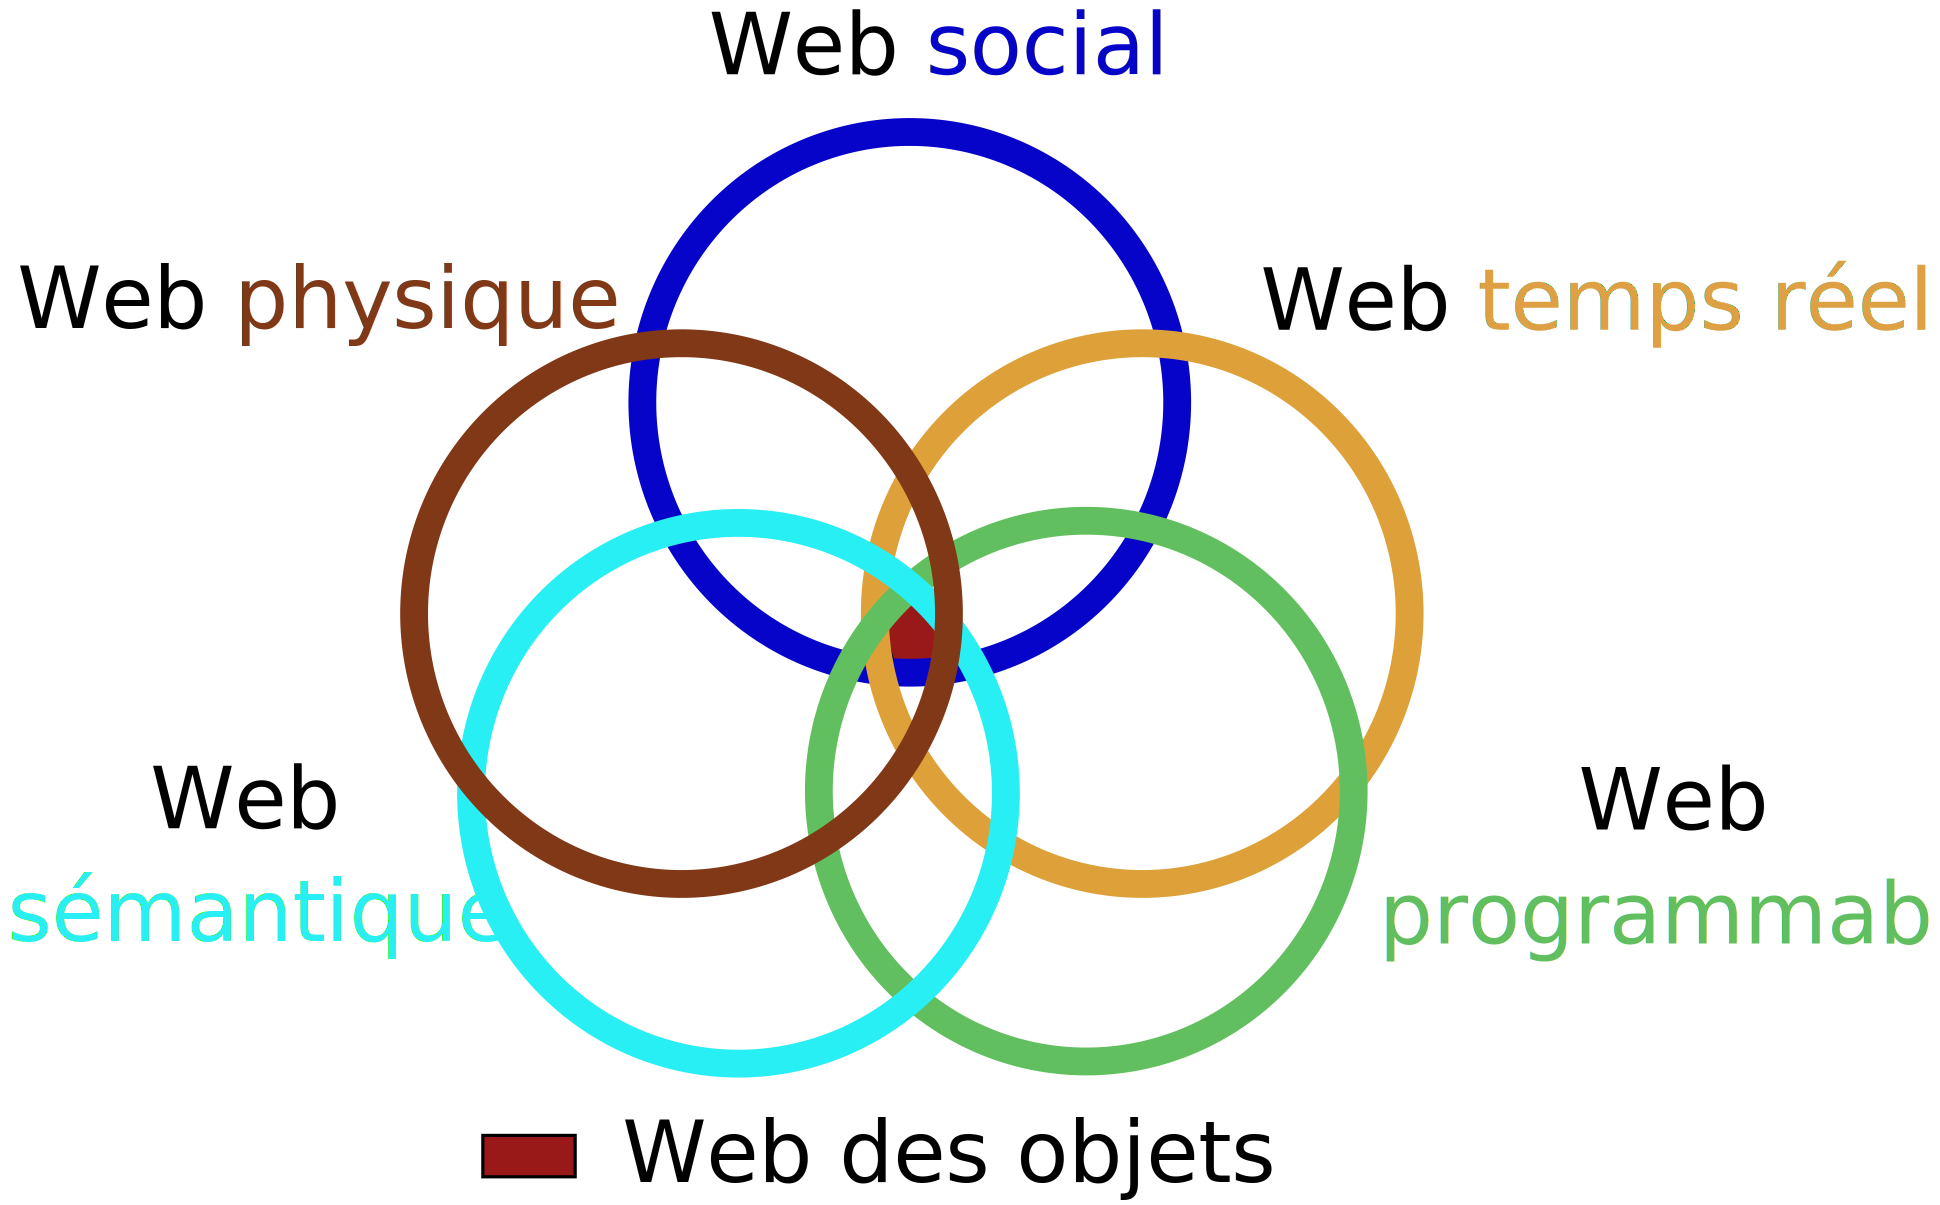
\includegraphics[width=\linewidth]{./Images/Chapter08/internet-objects.pdf}}%
\begin{jazzitemize}
\item \href{https://fr.wikipedia.org/wiki/Internet_des_objets}{Internet des objets.}.
\item \href{https://fr.wikipedia.org/wiki/S\%C3\%BBret\%C3\%A9_de_fonctionnement_des_syst\%C3\%A8mes_informatiques}{Sûreté.}.
\item \href{https://fr.wikipedia.org/wiki/S\%C3\%A9curit\%C3\%A9_des_syst\%C3\%A8mes_d'information}{Sécurité}.
\item \href{https://fr.wikipedia.org/wiki/Interactions_homme-machine}{Interface humain-machine}.
\end{jazzitemize}

\overparagraph{Ce que dit le programme}

\begin{tcolorbox}[title={Introduction}, toprule=0pt, leftrule=0pt, rightrule=0pt, arc=0pt,
                  fonttitle=\scshape\boxtitlefont,
                  colbacktitle=white, coltitle=firstcolor, colframe=firstcolor, colback=firstcolor!10,
                  breakable, enhanced jigsaw]


Embarquer l’informatique dans les objets a beaucoup d’avantages : simplifier leur fonctionnement, leur donner plus de possibilités d’usage et de sûreté et, leur permettre d’intégrer de nouvelles possibilités à matériel constant par simple modification de leur logiciel.

Après avoir transformé les chaînes de montage des automobiles et les avions dans les années quatre-vingt-dix, l’informatique intervient maintenant dans des domaines toujours plus nombreux : automobile, réseau ferroviaire et transports urbains, domotique, robotique, loisirs, etc., conduisant à un nouvel Internet des objets.

Pour les avions par exemple, l’informatique gère le vol en commandant finement des servomoteurs électriques, plus légers et plus fiables que les vérins hydrauliques, les réacteurs, la navigation et le pilotage automatique et, permet l’atterrissage automatique par temps de brouillard. Elle a eu un impact décisif sur l’amélioration de la sécurité aérienne.

Les objets informatisés avaient autrefois des \textit{interfaces homme-machine} (IHM) dédiées, souvent dépendantes d’une liaison filaire directe. Mais les technologies du Web intégrées au téléphone portable autorisent maintenant d’y rassembler les interfaces des objets du quotidien, ce qui en simplifie et uniformise l’usage. Les objets informatisés deviennent ainsi connectés.
\end{tcolorbox}

\begin{tcolorbox}[title={Impacts sur les pratiques humaines}, toprule=0pt, leftrule=0pt, rightrule=0pt, arc=0pt,
                  fonttitle=\scshape\boxtitlefont,
                  colbacktitle=white, coltitle=firstcolor, colframe=firstcolor, colback=firstcolor!10,
                  breakable, enhanced jigsaw]
L’impact de l’informatisation des objets devient considérable, surtout depuis que leurs interfaces s’unifient. Le but est de fabriquer des machines d’utilisation facile permettant des fonctionnalités améliorées, voire complètement nouvelles comme la voiture autonome. Celle-ci utilise à la fois des techniques de systèmes embarqués pour son fonctionnement et sa navigation et de l’intelligence artificielle pour l’analyse en temps-réel de l’environnement à l’aide de capteurs divers et variés (caméras, radars, lidars, etc.).

Comme l’informatique embarquée interagit avec le monde physique en exposant quelquefois des vies humaines ou des équipements critiques (réseaux électriques par exemple), elle est soumise à de fortes contraintes de sûreté (absence d’erreurs) et de sécurité (résistance aux attaques). En avionique, ferroviaire ou autres applications critiques, des processus lourds de certification externe sont utilisés. Cependant dans beaucoup de systèmes embarqués moins critiques, la sécurité reste souvent un point faible et les objets connectés sont de plus en plus utilisés comme robots pour lancer des attaques sur internet.
\end{tcolorbox}

\subsubsection[Volet historique]{Volet historique}
\label{subsub:VIII.3.1.2}

La notion d'Internet des objets\caution[t]<firstcolor>{%
Entre un \href{https://fr.wikipedia.org/wiki/Robot}{robot} et autre \href{https://fr.wikipedia.org/wiki/Internet_des_objets}{objet connecté}, le principe est le même, les deux classes d'objets comprennent trois types d'éléments constitutifs : des capteurs, des actionneurs et un programme qui permet à l'objet d'interagir avec l'environnement. On définit par ailleurs la \href{https://fr.wikipedia.org/wiki/Domotique}{\emph{domotique}} comme de l’informatique associée à des objets connectés du quotidien associés aux bâtiments, « l'habitat intelligent ».}{Note}
 résulte de la convergence de plusieurs technologies, de l'analyse en temps réel, de l'apprentissage automatique, des capteurs de produits de base et des systèmes intégrés. Les domaines traditionnels des systèmes embarqués, des réseaux de capteurs sans fil, des systèmes de contrôle, de l’automatisation (y compris l’automatisation de la maison et des bâtiments) et autres contribuent tous à l'activation de l'Internet des objets.

Le concept de réseau d'appareils intelligents a été discuté dès 1982 : un distributeur automatique de boisson modifié de l'Université Carnegie Mellon devenant le premier appareil connecté à Internet, capable de signaler ses stocks et de savoir si les boissons fraîchement chargées étaient froides ou non. L'article de 1991 de Mark \textsc{Weiser} sur l'informatique omniprésente, « L'ordinateur du XXI\frup{e} siècle », ainsi que des institutions académiques telles que \textsc{UbiComp} et \textsc{PerCom} ont produit la vision contemporaine de l'Internet des Objets. En 1994, Reza \textsc{Raji} a décrit le concept dans IEEE Spectrum comme « un [déplacement] de petits paquets de données vers un grand ensemble de nœuds, afin d'intégrer et d'automatiser tout, des appareils ménagers aux usines entières ». Entre 1993 et ​​1997, plusieurs sociétés ont proposé des solutions. Le domaine a pris de l'ampleur lorsque Bill \textsc{Joy} a envisagé la communication D2D (\textit{Device to Device}) dans le cadre de son cadre « Six Webs », présenté au Forum économique mondial de Davos en 1999.

Le terme « Internet des objets » a probablement été inventé par Kevin \textsc{Ashton} de \textsc{Procter \& Gamble}, futur centre d'identification automatique du MIT, en 1999, bien qu'il préfère l'expression « Internet pour les objets ». Un article de recherche mentionnant l'Internet des objets a été soumis à la conférence pour les chercheurs nordiques en Norvège, en juin 2002, précédée d'un article publié en finnois en janvier 2002. L’implémentation décrite ici a été développée par Kary \textsc{Främling} et son équipe de l’Université technologique de Helsinki et correspond plus étroitement à l’infrastructure moderne, c’est-à-dire une infrastructure de système d’information permettant la mise en œuvre d’objets connectés intelligents.

Définissant l'Internet des objets comme « simplement le moment où plus de choses ou d'objets étaient connectés à Internet que de personnes », \textsc{Cisco Systems} a estimé que l'Internet des objets était « né » entre 2008 et 2009, avec un ratio croissant d'objets par personnes de 0,08 en 2003 à 1,84 en 2010.

\noindent Sources : 
\href{https://en.wikipedia.org/wiki/Internet_of_things}{\textit{Internet of things} \faWikipediaW} ;
\href{https://fr.wikipedia.org/wiki/Internet_des_objets}{Internet des objets \faWikipediaW}.


\begin{jazzfigure*}
\Centering
\begin{tikzpicture}[scale=1, >=latex, inner sep=0pt, outer sep=0pt, label distance=2pt]
%\draw[step=0.25cm,style=help lines, line width=0.1pt] (0,0) grid (16.5,9);
%\draw[step=1cm,style=help lines, line width=0.8pt] (0,0) grid (16.5,9);
%-----
\draw[->,line width=1.6pt,secondcolor] (0.8pt,0) -- (16.5,8.25);
\draw[->,line width=1.6pt] (0,0) -- (16.5,0.0);
\draw[->,line width=1.6pt,xshift=0.8pt] (0,0) -- (0.0,9.0);
%---
\node[font=\footnotesize] at (1,-0.25) {2000};
\node[font=\footnotesize] at (6,-0.25) {2010};
\node[font=\footnotesize] at (11,-0.25) {2020};
\node[font=\small] at (15.5,-0.3333) {Temps};
\node[font=\small, anchor=west] at (0.3333,8.5) {Avancées technologiques};
%---
\node[draw=firstcolor, fill=white, line width=0.6pt, inner sep=2pt, font=\footnotesize, align=center] 
  at (2.5,1.25) {Étiquettes RFID pour faciliter\\ l'acheminement, l'inventaire\\ et la prévention des risques};
\node[draw=firstcolor, fill=white, line width=0.6pt, inner sep=2pt, font=\footnotesize, align=center] 
  at (6,3.0) {Surveillance, sécurité,\\ soins médicaux, transport,\\ sécurité alimentaire,\\ gestion de documents, etc.};
\node[draw=firstcolor, fill=white, line width=0.6pt, inner sep=2pt, font=\footnotesize, align=center] 
  at (9.0,4.5) {Localisation des personnes\\ et des objets du quotidien};
\node[draw=firstcolor, fill=white, line width=0.6pt, inner sep=2pt, font=\footnotesize, align=center] 
  at (12.0,6.0) {Téléopération et téléprésence :\\ capacité de surveiller\\ et contrôler des objets éloignés};
%---
\node[draw=none, fill=none, line width=0.6pt, inner sep=2pt, font=\footnotesize, align=center] 
  at (2.0,2.375) {Demande\\ de logistique accélérée};
\node[draw=none, fill=none, line width=0.6pt, inner sep=2pt, font=\footnotesize, align=center] 
  at (5.15,4.45) {Réduction des coûts\\ menant à la diffusion\\ d'une 2\frup{e} vague de demandes};
\node[draw=none, fill=none, line width=0.6pt, inner sep=2pt, font=\footnotesize, align=center] 
  at (7.75,5.675) {Capacité des dispositifs\\ intérieurs de recevoir\\ des signaux de géolocalisation};
\node[draw=none, fill=none, line width=0.6pt, inner sep=2pt, font=\footnotesize, align=center] 
  at (11.25,7.275) {Miniaturisation électronique\\ à économie d'énergie\\ et évantails de possibilités};
\node[draw=none, fill=none, line width=0.6pt, inner sep=2pt, font=\footnotesize, align=center] 
  at (14.25,8.5) {Fusion des agents logiciels\\ et des capteurs avancés};
%---
\node[draw=none, fill=none, inner sep=2pt, font=\footnotesize, align=center, anchor=west, text=secondcolor]
  at (4.65,1.25) {Aides pour la chaîne d'approvisionnement};
\node[draw=none, fill=none, inner sep=2pt, font=\footnotesize, align=center, anchor=west, text=secondcolor]
  at (8.0,3.0) {Demandes du marché vertical};
\node[draw=none, fill=none, inner sep=2pt, font=\footnotesize, align=center, anchor=west, text=secondcolor]
  at (11.0,4.5) {Positionnement omniprésent};
\node[draw=none, fill=none, inner sep=2pt, font=\footnotesize, align=center, anchor=west, text=secondcolor]
  at (14.25,6.0) {Réseaux\\ du\\ monde physique};
\end{tikzpicture}
\caption{\label{fig:VIII.1}Historique de la technologie : connectivité des choses (d'après SRI \textit{Consulting Business Intelligence}).}
\end{jazzfigure*}

\overparagraph*{Ce que dit le programme}

\begin{tcolorbox}[title={Repères historiques}, toprule=0pt, leftrule=0pt, rightrule=0pt, arc=0pt,
                  fonttitle=\scshape\boxtitlefont,
                  colbacktitle=white, coltitle=firstcolor, colframe=firstcolor, colback=firstcolor!10,
                  breakable, enhanced jigsaw]
\begin{jazzitemize}
\item 1967 : premier système embarqué de guidage lors de la mission lunaire \textsc{Apollo}.
\item 1971 : premier processeur produit par \textsc{Intel}.
\item 1984 : sortie de l’\textsc{Airbus} 320, premier avion équipé de commandes électriques informatisées. 
\item 1998 : mise en service du métro informatisé sans conducteur \textsc{Météor} (ligne 14 à Paris).
\item 1999 : introduction de l’expression « Internet des objets » par Kevin \textsc{Ashton}.
\item 2007 : arrivée du \textit{smartphone}.
\end{jazzitemize}

On estime à 50 milliards le nombre d’objets connectés en 2020.
\end{tcolorbox}

\subsubsection[Explication des notions]{Explication des notions}
\label{subsub:VIII.3.1.3}

\overparagraph{Idées-forces}

\begin{jazzitemize}
\item Pour programmer des objets connectés ou embarqués à l'intérieur d'un autre système, le paradigme de programmation de base est événementiel : ce sont les entrées des capteurs qui déclenchent des fonctions du code qui réagit et ajuste les sorties et son état interne.
\item Pour assurer la sûreté informatique, on travaille à la fois au niveau de la conception et de la vérification : la conception avec des langages de modélisation du système utilisé (comme UML)  et la vérification avec des méthodes formelles  qui travaillent sur la sémantique du programme pour en prédire le fonctionnement.
\item Mais ces méthodes prévisionnelles ne sont jamais complètes et c'est l'expérimentation qui permet de compléter la validation de tels systèmes. 
\item Pour assurer la sécurité des systèmes informatiques on utilise les mêmes méthodes que pour protéger un système classique : authentification des personnes ou des algorithmes qui accèdent à l'objet et chiffrage des données.
\end{jazzitemize}

\overparagraph{Mots-clefs}

\begin{jazzitemize}
\item \href{https://fr.wikipedia.org/wiki/Programmation_\%C3\%A9v\%C3\%A9nementielle}{Programmation événementielle} et \href{https://fr.wikipedia.org/wiki/Programmation_synchrone}{programmation synchrone}.
\item \href{https://fr.wikipedia.org/wiki/Internet_des_objets}{Internet des objets}.
\item \href{https://fr.wikipedia.org/wiki/S\%C3\%BBret\%C3\%A9_de_fonctionnement_des_syst\%C3\%A8mes_informatiques}{Sûreté}. 
\item \href{https://fr.wikipedia.org/wiki/S\%C3\%A9curit\%C3\%A9_des_syst\%C3\%A8mes_d'information}{Sécurité}.
\item \href{https://fr.wikipedia.org/wiki/Interactions_homme-machine}{Interface humain-machine}.
\end{jazzitemize}

\overparagraph{Ce que dit le programme}

\begin{tcolorbox}[title={Données et information}, toprule=0pt, leftrule=0pt, rightrule=0pt, arc=0pt,
                  fonttitle=\scshape\boxtitlefont,
                  colbacktitle=white, coltitle=firstcolor, colframe=firstcolor, colback=firstcolor!10,
                  breakable, enhanced jigsaw]
Dans les \emph{systèmes informatiques embarqués}, l’information provient soit des IHM soit des capteurs, pour contrôler automatiquement ou manuellement le fonctionnement physique par des actionneurs et transmettre des informations aux utilisateurs. Le flux d’informations à travers les IHM permet ainsi une interaction continue entre l’homme et la machine.
\end{tcolorbox}

\begin{tcolorbox}[title={Algorithmes et programmes}, toprule=0pt, leftrule=0pt, rightrule=0pt, arc=0pt,
                  fonttitle=\scshape\boxtitlefont,
                  colbacktitle=white, coltitle=firstcolor, colframe=firstcolor, colback=firstcolor!10,
                  breakable, enhanced jigsaw]
Le développement des logiciels embarqués est délicat, car il pose souvent des questions de temps-réel, c’est-à-dire de respect de temps de réponse imposé. Ceci conduit à des méthodes de programmation spécifiques.
\end{tcolorbox}

\begin{tcolorbox}[title={Machines}, toprule=0pt, leftrule=0pt, rightrule=0pt, arc=0pt,
                  fonttitle=\scshape\boxtitlefont,
                  colbacktitle=white, coltitle=firstcolor, colframe=firstcolor, colback=firstcolor!10,
                  breakable, enhanced jigsaw]
Les microprocesseurs sont beaucoup plus nombreux dans les objets que dans les ordinateurs et téléphones, mais ils sont souvent plus petits, moins chers et moins rapides. Les \emph{capteurs} et \emph{actionneurs} reposent sur des technologies physiques et électroniques variées, allant quelquefois vers l’électronique de puissance. Un problème essentiel est la réduction de la consommation électrique, surtout pour les appareils sur pile.
\end{tcolorbox}

\overparagraph{Web-conférence}

\begin{marginvideo}
	[\label{vid:VIII.6}Objets connectés, Jean-Philippe \textsc{Eneau}.]%
	%\movie[width=\marginparwidth,showcontrols]%
	%	{\includegraphics[width=\marginparwidth]{./Images/Pictograms/film-strip-dark-electric-blue.png}}%
	%	{./Videos/Chapter08/vidVIII-06-conf-snt-embedded-objects-jean-philippe-eneau.mp4}%
	\href{https://www.youtube.com/watch?v=JC2VCzYAnC8}%
	  {\includegraphics[width=\marginparwidth]{./Images/Pictograms/film-strip-dark-electric-blue.png}}%
	\launchvideo{https://www.youtube.com/watch?v=JC2VCzYAnC8}
\end{marginvideo}

\textsc{Class'Code} \textsc{Pays-de-Loire} a organisé des conférences qui abordent les sept thématiques du programme SNT. Leur objectif est de fournir une vue d’ensemble et de poser les bases nécessaires à l’appropriation de ces grands domaines sous deux angles définis par le programme :
\begin{itemize}
\item Une présentation historique (30 à 45 minutes) : grandes étapes de création/développement, acteurs majeurs, contexte général, histoire des idées et mise en contexte suffisamment fiable pour être réutilisée en cours.
\item Des exemples concrets de ce qui est étudié ou produit aujourd’hui dans ces domaines et une réflexion sur les besoins et enjeux actuels et à venir à travers un débat (45 à 60 minutes) qui laisse la parole à des personnes travaillant actuellement dans ces champs de spécialité  (chercheurs, enseignants, étudiants, entreprises...), que ce soit en recherche ou en entreprise.
\end{itemize}

La conférence sur l'Informatique embarquée et les objets connectés a eu lieu le 21 mars 2019 dans le cadre du projet \textsc{Class'Code} à l’Université de Nantes.

\begin{gofurther}{Ressources complémentaires}
\lightbf{Se former}
\begin{itemize}\jazzitem
\item Introduction aux \href{https://pixees.fr/interfacer-la-machine-a-lhumain-2/}{interfaces humain-machine}.
\item Cours introductif à l'\href{http://www.lirmm.fr/~seriai/uploads/Enseignement/iot.pdf}{Internet des objets}.
\item Pour les enseignants : la \href{https://magistere.education.fr/dgesco/}{conférence de Pascale \textsc{Costa} l'nformatique embarquée et objets connectés et aussi localisation, cartographie et mobilité}, lors des formations nationales, accès par m@gistere (réservé aux enseignant·e·s).
\item Une \href{https://interstices.info/dossier/snt-informatique-embarquee-et-objets-connectes/}{sélection d'articles} du site \textsc{Interstices}.
\end{itemize}

\vspace{2pt}
\lightbf{Créer son cours}
\begin{itemize}\jazzitem
\item \href{./Documents/Chapter08/cardVIII-18-snt-iot-ihm-nicolas-tourreau.odt}{Fiche de connaissance} sur les IHM par \href{mailto://ntourreau@ac-toulouse.fr}{Nicolas \textsc{Tourreau}}, validée sur \href{mailto://sciences-numeriques-technologie@groupes.renater.fr}{Sciences numériques technologie}.
\item \href{https://pixees.fr/quest-ce-que-la-securite-et-la-surete-informatique/}{Qu’est-ce que la sécurité et la sûreté informatique ?}
\item L'\href{https://books.openedition.org/editionsmsh/78}{\textit{Internet des objets}}, livre ouvert consultable en ligne.
\item \href{https://www.framboise314.fr/publications-revues-magazines-livres-e-books-et-articles-sur-le-raspberry-pi/the-magpi/}{Revue en ligne} avec beaucoup de pistes librement réutilisables concernant le \textsc{Raspberry-Pi}.
\item \href{https://pixees.fr/demonter-un-ordinateur/}{Démonter un ordinateur}.
\item \href{https://pixees.fr/monter-un-ordinateur/}{Monter un ordinateur}.
\item \href{https://www.f-legrand.fr/scidoc/docimg/sciphys/arduino/python/python.html}{\textit{Framework}} pour travailler sur \textsc{Arduino} en \textsc{Python}. Possibilité d'utiliser le \href{http://tableauxmaths.fr/spip/spip.php?article149}{\textsc{GUI Kivy}} pour créer une IHM qui pilote \textsc{Arduino}.
\end{itemize}
\end{gofurther}


\subsection[Réaliser des activités]{Réaliser des activités}
\label{sub:VIII.3.2}

\overparagraph*{Exemple d'activités}

Les activités proposées\caution[t]<firstcolor>{%
Toutes les fiches actuellement collectées sont disponibles à l'URL : \url{http://tinyurl.com/yx9qce8s} et on peut aussi proposer des activités.}{Note de la rédaction}
sont disponibles sous forme de fiches à télécharger (format ODT de la suite bureautique libre \textsc{LibreOffice}).

\begin{jazzitemize}
\item \textdoc{./Documents/Chapter08/cardVIII-19-snt-ihm-david-roche.odt}{Introduction aux interfaces « homme - machine »}.
\item \textdoc{./Documents/Chapter08/cardVIII-20-snt-voiture-autonome-david-roche.odt}{Introduction aux principes de la voiture autonome}.
\item \textdoc{./Documents/Chapter08/cardVIII-21-snt-robot-david-roche.odt}{Découverte de la robotique et réflexion sur son impact au travail}.
\item \textdoc{./Documents/Chapter08/cardVIII-22-snt-robot-thymio-david-roche.odt}{Programmer un robot pédagogique (capteurs et actionneurs)}.
\end{jazzitemize}

\noindent Fiche d'activité élève :
\begin{jazzitemize}
\item \pdfdoc{./Documents/Chapter08/activityVIII-04-smartphone-appinventor.pdf}{\textit{Smartphone} et \textsc{App Inventor}}.
\end{jazzitemize}

%\overparagraph{Ce que propose le programme}

\begin{tcolorbox}[title={Ce que propose le programme}, toprule=0pt, leftrule=0pt, rightrule=0pt, arc=0pt,
                  fonttitle=\scshape\boxtitlefont,
                  colbacktitle=white, coltitle=firstcolor, colframe=firstcolor, colback=firstcolor!10,
                  breakable, enhanced jigsaw]
\begin{jazzitemize}
\item Identifier les évolutions apportées par les algorithmes au contrôle des freins et du moteur d’une automobile, ou à celui de l’assistance au pédalage d’un vélo électrique.   
\item Réaliser une IHM pouvant piloter deux ou trois actionneurs et acquérir les données d’un ou deux capteurs. 
\item Gérer des entrées/sorties à travers les ports du système. 
\item Utiliser un tableau de correspondance entre caractères envoyés ou reçus et commandes physiques (exemple : le moteur A est piloté à 50\% de sa vitesse maximale lorsque le robot reçoit la chaîne de caractères « A50 »).
\end{jazzitemize}
\end{tcolorbox}


%----------
\section[Localisation et cartographie]{Localisation et cartographie}
\label{sec:VIII.4}


\subsection[Découvrir la thématique]{Découvrir la thématique}
\label{sub:VIII.4.1}

\subsubsection[Ancrage dans le réel]{Ancrage dans le réel}
\label{subsub:VIII.4.1.1}

\overparagraph{Points-clefs}

\begin{marginvideo}
	[\label{vid:VIII.7}Localisation et cartographie.]%
	%\movie[width=\marginparwidth,showcontrols]%
	%	{\includegraphics[width=\marginparwidth]{./Images/Pictograms/film-strip-dark-electric-blue.png}}%
	%	{./Videos/Chapter08/vidVIII-07-mooc-snt-localization.mp4}%
	\href{https://www.youtube.com/watch?v=iTfNhcC2vBA}%
	  {\includegraphics[width=\marginparwidth]{./Images/Pictograms/film-strip-dark-electric-blue.png}}%
	\launchvideo{https://www.youtube.com/watch?v=iTfNhcC2vBA}
\end{marginvideo}

\begin{jazzitemize}
\item Une carte est un outil de représentation d'informations hiérarchisées liées à une localisation.  Les cartes permettent de combiner différentes informations,  pour visualiser des réalités aussi diverses que le développement d'un territoire ou la propagation d'une maladie.
\item Le fait que nous soyons aujourd'hui localisé·e·s en permanence a des conséquences importantes sur notre vie quotidienne : cela permet d'être aidé en cas de situation critique, mais aussi d'être repéré à tout moment qu'on le souhaite ou non.
\item La localisation est incontournable, et pas uniquement au niveau de notre \textit{smartphone} : dès que nous interagissons avec un système numérique, nous sommes localisés, et le fait de ne plus se faire localiser à un moment donné est en soi une information.
\end{jazzitemize}

\overparagraph{Mots-clefs}

\begin{jazzitemize}
\item \href{https://fr.wikipedia.org/wiki/G\%C3\%A9olocalisation}{Géolocalisation}.
\item \href{https://fr.wikipedia.org/wiki/GPS_(assistant_de_navigation)}{Assistant de navigation}.
\item \href{https://fr.wikipedia.org/wiki/G\%C3\%A9omatique}{Géomatique}.
\end{jazzitemize}

%\vspace*{-\baselineskip}
%\sidegraphic[Géolocalisation.]{\includegraphics[width=\linewidth]{./Images/Chapter08/geolocation.png}}%
\overparagraph{Ce que dit le programme}

\begin{tcolorbox}[title={Introduction}, toprule=0pt, leftrule=0pt, rightrule=0pt, arc=0pt,
                  fonttitle=\scshape\boxtitlefont,
                  colbacktitle=white, coltitle=firstcolor, colframe=firstcolor, colback=firstcolor!10,
                  breakable, enhanced jigsaw]
La cartographie est essentielle pour beaucoup d’activités : agriculture, urbanisme, transports, loisirs, etc. Elle a été révolutionnée par l’arrivée des cartes numériques accessibles depuis les ordinateurs, tablettes et téléphones, bien plus souples à l’usage que les cartes papier.

Les \emph{cartes numériques} rassemblent toutes les échelles et permettent de montrer différents aspects de la région visualisée sur une seule carte. Les algorithmes de recherche permettent de retrouver sur la carte les endroits en donnant simplement leur nom, et de calculer des itinéraires entre points selon des modes de transports variés.
\end{tcolorbox}

\begin{tcolorbox}[title={Impacts sur les pratiques humaines}, toprule=0pt, leftrule=0pt, rightrule=0pt, arc=0pt,
                  fonttitle=\scshape\boxtitlefont,
                  colbacktitle=white, coltitle=firstcolor, colframe=firstcolor, colback=firstcolor!10,
                  breakable, enhanced jigsaw]
Les cartes numériques, accessibles depuis un téléphone, remplacent progressivement les cartes sur papier. Leurs interfaces permettent d’accéder commodément à de nombreux types d’information. Couplé aux algorithmes de calculs d’itinéraires, le GPS est utilisé systématiquement pour les transports, l’agriculture, la randonnée, la navigation à voile, etc.

Le maintien à jour des cartes numériques est un problème difficile qui demande beaucoup de ressources au plan mondial. Les erreurs dans les cartes, inévitables à cause de l’énorme quantité d’informations à collecter et à traiter, peuvent avoir des conséquences dramatiques.

Par ailleurs, de nombreuses applications ont accès à la localisation dans un téléphone, ce qui leur permet d’envoyer des publicités non désirées, de suivre vos itinéraires, ou de localiser une personne. Enfin, le GPS n’est pas toujours sûr, car facile à brouiller à l’aide d’appareils simples.
\end{tcolorbox}

\subsubsection[Volet historique]{Volet historique}
\label{subsub:VIII.4.1.2}

\sidegraphic[Carte/\href{https://fr.wikipedia.org/wiki/Rocher_1_de_Bedolina}{rocher de Bedolina}.]{\includegraphics[width=\linewidth]{graphVIII-05-mappa-di-bedolina-luca-giarelli.jpg}}%
Les premières cartes connues représentent les étoiles et non la terre. Des points datés de 16\,500 BC, trouvés sur les murs de la grotte de Lascaux montrent une partie du ciel nocturne, incluant trois des étoiles les plus brillantes, Véga, Deneb, et Altaïr (le Triangle d'été), ainsi que l'amas d'étoiles les Pléiades. La grotte du Castillo en Espagne possède également une carte de la Couronne boréale datée de 12\,000 BC. 

Depuis l'Antiquité, jusqu'au milieu du XVI\frup{e} siècle, les relevés sont issus de témoignages. Les premières mises en forme « scientifiques~» datent du II\frup{e} siècle après notre ère avec la cartographie de \textsc{Ptolémée} (150), où celui-ci énonce quelques précautions pour dessiner une carte sur un plan. Par la suite les relevés sont assemblés par des cartogra\-phes experts et alimentés par les premiers essais de statistiques rassemblés par les représentants de l'autorité (époque antique romaine, des moines savants du Moyen Âge puis des grandes découvertes). Les supports utilisés --- notamment les cartes marines --- sont grossières car elles ne respectent ni les angles, ni les distances réelles. 

Le véritable développement intervient avec l'amélioration des outils de mesure mis au point par la géodésie et les géomètres, ainsi que l'amélioration des registres de tous types, devenant de larges sources statistiques. Aussi, les traits et les données s'affinent. Ainsi les premières mesures astronomiques (longitudes et latitudes) de localités de la France effectuées par Jean \textsc{Picard} commencées en 1671, permettent à \textsc{La Hire} d'établir en 1682 une carte corrigée qui affine le contour du littoral et réduit considérablement les vraies proportions de la France.

\sidegraphic[Quartiers de Paris.]{\includegraphics[width=\linewidth]{graphVIII-06-mapfr.jpg}}%
L’une des premières applications connues de l’analyse cartographi\-que concernait le domaine de l’épidémiologie avec, en 1832, la publication du « Rapport sur la marche et les effets du choléra dans Paris et le département de la Seine », rédigé par le géographe français Charles \textsc{Picquet}. Ce dernier a représenté les quarante-huit districts de la ville de Paris. Il a utilisé un système de coloris dégradé en fonction du pourcentage de décès par le choléra pour mille habitants.

L'utilisation des engins aéronautiques (dirigeables, avions, hélicoptères) à partir du début du XX\frup{e} siècle permet d'affiner et de mettre à jour plus rapidement la couverture cartographique, mais pour des espaces à chaque fois relativement limités et concernant presque uniquement les terres émergées. Dans la dernière partie du XX\frup{e} siècle, un pas technique majeur est franchi avec l'utilisation et le traitement numérique des ondes émises par des satellites : les contours terrestres sont alors pour la première fois photographiés depuis le ciel. Des cartographies du fond des océans ou des zones inaccessibles deviennent beaucoup plus précises. La cartographie complète de la Lune et de Mars est réalisée grâce aux satellites d'exploration ou sondes spatiales. 

Grâce à des avancées mathématiques et informatiques, on obtient avec facilité toujours plus de projections planes innovantes, qui doivent toujours arbitrer entre conservation des parallèles, des aires, et des longueurs. Des cartes amorphes (cartogrammes) sont aussi apparues. Le support digital permet la duplication, le transfert à bas coût, et le traitement automatisé (par exemple le projet \href{https://fr.wikipedia.org/wiki/Corine_Land_Cover}{Corine Land Cover} pour l'aménagement du territoire).

\sidegraphic[Carte topographique de l'île de Corfou, données satellitaires.]{\includegraphics[width=\linewidth]{graphVIII-07-corfu-topographic-map-fr.pdf}}%
Un autre apport du numérique concerne la capacité à mettre en relation et diffuser des documents d'intérêt cartographique du monde entier et de toutes les époques, \textit{via} Internet. En France, un Consortium intitulé « Cartes et photographies pour les géographes » vise  à faciliter le tournant numérique de la recherche en sciences humaines et sociales, en développant le réseau de portails cartographiques et de plateformes de diffusion de données et métadonnées peu à peu mis en place, essentiellement par de grandes institutions, pour « généraliser l’accès à d’autres fonds pertinents et améliorer la diffusion des images géographiques » afin de « rendre accessibles, consultables et mobilisables des données cartographiques et photographiques nombreuses et éparses, qui constituent des fonds de laboratoires de recherche, de bibliothèques remarquables ou des fonds de chercheurs… » . Un mouvement de libération des données (\textit{Open data}) est également en cours qui, avec des organisations comme \href{https://www.openstreetmap.fr/}{\textsc{OpenStreetMap}}, devrait permettre de largement développer la cartographie historique et collaborative.

\noindent Source : \href{https://fr.wikipedia.org/wiki/Cartographie}{Cartographie \faWikipediaW} ; \href{https://fr.wikipedia.org/wiki/Syst\%C3\%A8me_d\%27information_g\%C3\%A9ographique}{Système d'information géographique \faWikipediaW}.

\overparagraph*{Ce que dit le programme}

\begin{tcolorbox}[title={Repères historiques}, toprule=0pt, leftrule=0pt, rightrule=0pt, arc=0pt,
                  fonttitle=\scshape\boxtitlefont,
                  colbacktitle=white, coltitle=firstcolor, colframe=firstcolor, colback=firstcolor!10,
                  breakable, enhanced jigsaw]
Les cartes ont été systématiquement numérisées à la fin du XX\frup{e} siècle.
Le principal instrument de localisation, GPS (\textit{Global Positioning System}), a été conçu par l’armée américaine dans les années soixante. Le premier satellite GPS fut lancé en 1978. Il y en a actuellement une trentaine, de sorte qu’à tout moment quatre à six satellites au moins sont visibles depuis tout point de la Terre. Couplé aux cartes numériques, le système GPS permet de se situer. Il n’est pas toujours efficace en ville, et peut être complété par d’autres moyens de localisation comme la détection de bornes Wi-Fi proches. D’autres systèmes plus précis, dont \textsc{Galileo}, sont en cours de déploiement.
\end{tcolorbox}

\vspace{4pt}
\begin{fullwidth}
\Centering
%\includegraphics[width=\linewidth]{map-steve-buissinne-pixabay.jpg}
\includegraphics[width=\linewidth]{gps-world-digital-designer-pixabay.png}
\end{fullwidth}


\subsubsection[Explication des notions]{Explication des notions}
\label{subsub:VIII.4.1.3}

\overparagraph{Idées-forces}

\begin{jazzitemize}
\item La localisation par satellite impose de recevoir quatre mesures,  car il y a quatre inconnues : trois spatiales et une temporelle.
\item Le calcul d'itinéraire correspond à un algorithme de calcul de plus court chemin (théorie des graphes), il est utilisé dans d'autres applications qui cherchent à trouver une suite d'étapes pour passer d'un état initial à un état final.
\item Une carte numérique n'est pas une image matricielle, mais une image vectorielle ce qui permet de la représenter à n'importe quelle échelle, et d'y adosser toutes sortes d'informations.
\end{jazzitemize}

\overparagraph{Mots-clefs}

\begin{jazzitemize}
\item \href{https://fr.wikipedia.org/wiki/Programmation_\%C3\%A9v\%C3\%A9nementielle}{Système d'information géographique (\textsc{Sig})}.
\item \href{https://fr.wikipedia.org/wiki/Internet_des_objets}{Système de positionnement par satellite}.
\end{jazzitemize}

\vfill

\overparagraph{Ce que dit le programme}

%\pagebreak

\begin{tcolorbox}[title={Données et information}, toprule=0pt, leftrule=0pt, rightrule=0pt, arc=0pt,
                  fonttitle=\scshape\boxtitlefont,
                  colbacktitle=white, coltitle=firstcolor, colframe=firstcolor, colback=firstcolor!10,
                  breakable, enhanced jigsaw]
Les informations des cartes numériques proviennent de nombreuses sources : services géographiques des États, photos prises par des satellites, avions ou voitures, données fournies par les utilisateurs, etc. Ces informations sont de natures diverses : topographiques, géologiques, photographiques, liées aux transports, à l’activité industrielle ou touristique, etc. Des projets collaboratifs comme \textsc{OpenStreetMap} permettent à chaque utilisateur d’ajouter des informations à une carte en libre accès, qui deviennent alors visibles par tous les utilisateurs.

Un satellite GPS contient des horloges atomiques mesurant le temps à une très grande précision et envoyant régulièrement des messages contenant cette heure. Chaque message se propageant à la vitesse de la lumière, le récepteur peut calculer sa distance au satellite. On peut en déduire sa position en suivant plusieurs satellites, ce que fait automatiquement le récepteur GPS.
\end{tcolorbox}

\begin{tcolorbox}[title={Algorithmes et programmes}, toprule=0pt, leftrule=0pt, rightrule=0pt, arc=0pt,
                  fonttitle=\scshape\boxtitlefont,
                  colbacktitle=white, coltitle=firstcolor, colframe=firstcolor, colback=firstcolor!10,
                  breakable, enhanced jigsaw]
Les algorithmes cartographiques concernent principalement l’affichage sélectif d’­­­­­informations variées et le \emph{calcul d’itinéraires}. L’affichage est paramétré par les informations à montrer, que l’on peut choisir par simples clics. Une difficulté est liée au mélange d’informations de types différents lors des changements d’échelle : les graphismes peuvent être très différents et beaucoup d’informations doivent être supprimées pour les grandes échelles, mais une route doit être représentée avec à peu près la même largeur, quelle que soit l’échelle.

Les récepteurs GPS fournissent la localisation sous une forme normalisée facilement décodable, par exemple selon le \emph{protocole NMEA 0183} (\textit{National Marine Electronics Association}), ou directement dans les métadonnées EXIF d’une photo. La localisation et les cartes se couplent dans le suivi permanent de la position sur la carte ou sur un itinéraire précalculé.
\end{tcolorbox}

\begin{tcolorbox}[title={Machines}, toprule=0pt, leftrule=0pt, rightrule=0pt, arc=0pt,
                  fonttitle=\scshape\boxtitlefont,
                  colbacktitle=white, coltitle=firstcolor, colframe=firstcolor, colback=firstcolor!10,
                  breakable, enhanced jigsaw]
Les machines utilisées pour la cartographie sont surtout les ordinateurs, tablettes et téléphones classiques équipés d’une application \textit{ad hoc}. Les récepteurs GPS spécialisés restent importants pour la navigation maritime ou aérienne, mais ceux pour la randonnée pédestre sont en voie de disparition, supplantés par les téléphones.

L’heure fournie par le GPS sert aussi de base pour la synchronisation précise des horloges internes des ordinateurs connectés à internet, ce qui est très important pour tous les échanges d’informations.
\end{tcolorbox}

\overparagraph{Web-conférence}

\begin{marginvideo}
	[\label{vid:VIII.8}Localisation cartographie et mobilité, Daniel \textsc{Bourreau}.]%
	%\movie[width=\marginparwidth,showcontrols]%
	%	{\includegraphics[width=\marginparwidth]{./Images/Pictograms/film-strip-dark-electric-blue.png}}%
	%	{./Videos/Chapter08/vidVIII-08-conf-snt-localization-daniel-bourreau.mp4}%
	\href{https://www.youtube.com/watch?v=r2YwShs1QjA}%
	  {\includegraphics[width=\marginparwidth]{./Images/Pictograms/film-strip-dark-electric-blue.png}}%
	\launchvideo{https://www.youtube.com/watch?v=r2YwShs1QjA}
\end{marginvideo}

\textsc{Class'Code} \textsc{Pays-de-Loire} a organisé des conférences qui abordent les sept thématiques du programme SNT. Leur objectif est de fournir une vue d’ensemble et de poser les bases nécessaires à l’appropriation de ces grands domaines sous deux angles définis par le programme :
\begin{itemize}
\item Une présentation historique (30 à 45 minutes) : grandes étapes de création/développement, acteurs majeurs, contexte général, histoire des idées et mise en contexte suffisamment fiable pour être réutilisée en cours.
\item Des exemples concrets de ce qui est étudié ou produit aujourd’hui dans ces domaines et une réflexion sur les besoins et enjeux actuels et à venir à travers un débat (45 à 60 minutes) qui laisse la parole à des personnes travaillant actuellement dans ces champs de spécialité  (chercheurs, enseignants, étudiants, entreprises...), que ce soit en recherche ou en entreprise.
\end{itemize}

La conférence sur la \textit{localisation, cartographie et mobilité} a eu lieu le 14 mars 2019 dans le cadre du projet \textsc{Class'Code} à l’Université de Nantes. Elle a été retransmise en ligne et est maintenant disponible sur \textsc{YouTube}.

\begin{gofurther}{Ressources complémentaires}
\lightbf{Se former}
\begin{itemize}\jazzitem
\item Une vidéo pour \href{https://pixees.fr/marier-geographie-et-informatique/}{découvrir la géomatique} (partageable avec les élèves).
\item Une \href{https://jeunes.cnes.fr/fr/tu-pris-ton-galileo}{vidéo explicative du CNES sur le fonctionnement de Galiléo}  (partageable avec les élèves).
\item Pour les enseignants : la \href{https://magistere.education.fr/dgesco/}{conférence de Pascale \textsc{Costa} l'nformatique embarquée et objets connectés et aussi localisation, cartographie et mobilité}, lors des formations nationales, accès par m@gistere (réservé aux enseignant·e·s).
\item Une \href{https://interstices.info/dossier/snt-localisation-cartographie-et-mobilite/}{sélection d'articles} du site \textsc{Interstices}.
\end{itemize}

\vspace{2pt}
\lightbf{Créer son cours}
\begin{itemize}\jazzitem
\item \href{./Documents/Chapter08/cardVIII-23-snt-gps-nicolas-tourreau.odt}{Fiche de connaissance sur le GPS} par \href{mailto://ntourreau@ac-toulouse.fr}{Nicolas \textsc{Tourreau}}, validée sur \href{mailto://sciences-numeriques-technologie@groupes.renater.fr}{Sciences numériques technologie}.
\item \href{./Documents/Chapter08/cardVIII-24-snt-map-nicolas-tourreau.odt}{Fiche de connaissance sur les cartes numériques} par \href{mailto://ntourreau@ac-toulouse.fr}{Nicolas \textsc{Tourreau}}, validée sur \href{mailto://sciences-numeriques-technologie@groupes.renater.fr}{Sciences numériques technologie}.
\item La \href{https://www.isoloir.net/}{ressource librement utilisable « isoloir »} propose une activité sur la localisation à faire en classe en semi-autonomie, ces \href{https://pixees.fr/informatique-et-societe-du-jeu-serieux-au-document-pedagogique/}{documents} sont librement réutilisables.
\item Le \href{https://streaming.ensg.eu/geodesie/portail/co/portail.html}{portail de vidéos de Géodésie générale} (Cours ENSG - Serge Botton – décembre 2013).
\item Une \href{http://cours-fad-public.ensg.eu/course/view.php?id=86}{approche calculatoire du positionnement d'un récepteur GNSS} à partir des observations de code C/A et de phase de trois constellations, sous \textsc{Matlab} ou \textsc{Octave}, Clément \textsc{Fontaine} et Jacques \textsc{Beilin}.
\item \href{http://cours-fad-public.ensg.eu/course/view.php?id=73}{Cours sur l'utilisation de la Théorie des graphes en géomatique} avec les contenus suivants : définitions de base, notions utiles, Stéphane \textsc{Pelle}.
\item Une vidéo rigolote sur la \href{https://leblob.fr/techno/la-geolocalisation}{géolocalisation} qui fait partie de la série \href{https://leblob.fr/series/jacques-dit}{\textsc{Jacques} a dit} et reste très attractive, malgré quelques approximations scientifiques, intéressantes du reste à faire débusquer par les élèves.
\item Articles de presse : \href{http://www.isnea.eu/le-suivi-par-gelocalisation-des-sarcelles-dhiver-un-defi-prometteur/}{Le suivi par géolocalisation des sarcelles d’hiver : un défi prometteur !} et \href{https://www.lesnumeriques.com/voiture/cartographie-hd-element-cle-voiture-autonome-a3501.html}{La cartographie HD, élément-clé de la voiture autonome}.
\item Il est possible de travailler sur \href{https://pypi.org/project/osmapi/}{\textsc{osmapi}} ou aussi d'utiliser la bibliothèque \textsc{Python} \href{https://github.com/python-visualization/folium}{\textsc{folium}} qui permet de travailler sur des cartes et d'obtenir le rendu dans un navigateur Web.
\end{itemize}
\end{gofurther}


\subsection[Réaliser des activités]{Réaliser des activités}
\label{sub:VIII.4.2}

\overparagraph*{Exemple d'activités}

Les activités proposées\caution[t]<firstcolor>{%
Toutes les fiches actuellement collectées sont disponibles à l'URL : \url{http://tinyurl.com/yx9qce8s} et on peut aussi proposer des activités.}{Note de la rédaction}
sont disponibles sous forme de fiches à télécharger (format ODT de la suite bureautique libre \textsc{LibreOffice}).

\begin{jazzitemize}
\item \textdoc{./Documents/Chapter08/cardVIII-25-snt-map-david-fialaire.odt}{Localisation, cartographie et mobilité (itinéraires)}.
\item \textdoc{./Documents/Chapter08/cardVIII-26-snt-map-gps-david-roche.odt}{Principe du GPS et de \textsc{Galileo}}.
\item \textdoc{./Documents/Chapter08/cardVIII-27-snt-openstreetmap-david-roche.odt}{Présentation du projet \textsc{OpenStreetMap} et contribution}.
\item \textdoc{./Documents/Chapter08/cardVIII-28-snt-map-python-gps-david-roche.odt}{Carte personnalisée avec \textsc{Python} et la bibliothèque \textsc{folium}}.
\item \textdoc{./Documents/Chapter08/cardVIII-29-snt-map-python-gps-david-roche.odt}{Principe de l’algorithme de \textsc{Dijkstra} ; création d’un itinéraire à l’aide de la bibliothèque \textsc{Python} \textsc{pyroutelib3}}.
\item \textdoc{./Documents/Chapter08/cardVIII-30-gps-quiz-pascal-barbier.odt}{Apprendre un élément du cours à travers la réalisation d'un quiz}.
\item \textdoc{./Documents/Chapter08/cardVIII-31-exif-gps-laurent-mathieu.odt}{Précision verticale des coordonnées GPS}.
\end{jazzitemize}

\noindent Fiche d'activité élève :
\begin{jazzitemize}
\item \pdfdoc{./Documents/Chapter08/activityVIII-05-snt-map.pdf}{Utilisation de \textsc{Géoportail}.}.
\end{jazzitemize}

%\overparagraph{Ce que propose le programme}

\begin{tcolorbox}[title={Ce que propose le programme}, toprule=0pt, leftrule=0pt, rightrule=0pt, arc=0pt,
                  fonttitle=\scshape\boxtitlefont,
                  colbacktitle=white, coltitle=firstcolor, colframe=firstcolor, colback=firstcolor!10,
                  breakable, enhanced jigsaw]
\begin{jazzitemize}
\item Expérimenter la sélection d’informations à afficher et l’impact sur le changement d’échelle de cartes (\textsc{GéoPortail}), ainsi que les ajouts d’informations par les utilisateurs \textsc{OpenStreetMap}.   
\item Mettre en évidence les problèmes liés à un changement d’échelle dans la représentation par exemple des routes ou de leur nom sur une carte numérique pour illustrer l’aspect discret du zoom. 
\item Calculer un itinéraire routier entre deux points à partir d’une carte numérique. 
\item Connecter un récepteur GPS sur un ordinateur afin de récupérer la trame NMEA, en extraire la localisation.
\item Extraire la géolocalisation des métadonnées d’une photo.
\item Situer sur une carte numérique la position récupérée.
\item Consulter et gérer son historique de géolocalisation. 
\end{jazzitemize}
\end{tcolorbox}

\begin{jazztable*}
\caption{\label{tab:VIII.1}Géolocalisation : compétences attendues chez les élèves.}
\Centering
\begingroup
\small
\renewcommand*{\arraystretch}{1.6}
\rowcolors{2}{tableLineOne}{tableLineTwo}
\begin{tabularx}{\linewidth}{lX}
\rowcolor{secondcolor}
\multicolumn{2}{c}{\Gape[6pt]{\textcolor{white}{\textbf{Géolocalisation}}}} \\
\rowcolor{firstcolor}
\multicolumn{1}{c}{\scshape\titlingfont\textcolor{white}{Contenus}} 
	&	\multicolumn{1}{c}{\scshape\titlingfont\textcolor{white}{Capacités attendues}} \\
GPS, \textsc{Galileo}
  & Décrire le principe de fonctionnement de la géolocalisation. \\
Cartes  numériques 
  & Identifier les différentes couches d’information de \textsc{GéoPortail} pour extraire différents types de données.
    Contribuer à \textsc{OpenStreetMap} de façon collaborative.\\
Protocole NMEA 0183 &
  Décoder une trame NMEA pour trouver des coordonnées géographiques. \\
Calculs d’itinéraires &
  Utiliser un logiciel pour calculer un itinéraire.
  Représenter un calcul d’itinéraire comme un problème sur un graphe. \\
Confidentialité &
  Régler les paramètres de confidentialité d’un téléphone pour partager ou non sa position.
\end{tabularx}% "%" est nécessaire pour éviter une alerte "underfull box"
\endgroup
\end{jazztable*}



%----------
\section[Que faire de ces ressources ? Quiz]{Que faire de ces ressources ? Autoévaluation}
\label{sec:VIII.5}

Les questionnaires\caution[t]<firstcolor>{%
La présentation des quiz du document\linebreak suit plus ou moins celle de la platefor\-me \textsc{Fun-Mooc}. La fonctionnalité manquante --- pas encore implémentée dans l'extension de style \LaTeX{} usitée --- est relative à la comptabilisation des points et à leur enregistrement. Aussi, il appartient au lecteur de jouer le jeu dans l'auto\-évaluation de ses connaissances.}{Note de la rédaction}
à choix multiple%
\parnote{De manière traditionnelle en \textsc{Ihm}, lorsqu'une seule réponse est correcte, les propositions sont précédées d'un cercle à cocher (\emph{radio button}) ; en revanche, dans le cas de plusieurs solutions possibles, il s'agit de carrés (\emph{check box}). En outre, après validation des réponses (« Vérifier »), leur explication s'affiche en marge ou infobulle (« Afficher la réponse »).}
--- QCM --- à suivre clôturent le présent chapitre \qnameref{chap:VIII} et correspondent à chaque sujet qui y est abordé.
\parnotes

\vspace{6pt}

\begin{quiz}[title={Données et traitements}]
\vspace{-\baselineskip}
\begin{quizquestion}[b]{1}{2}{Bien rivaux}
<Le disque vinyle est un bien rival parce que c'est un objet qu'on ne peut recopier, à l'inverse une vidéo numérique est un bien non rival puisque la copier ne coûte quasiment rien et n'affecte pas le bien initial.>
Parmi ces exemples, le/lesquels est/sont des biens rivaux ?
\points{1}
	\mcqproposal{Un des disques vinyles (produit à plus d’un million d’exemplaires) de la chanson « Que je t’aime » de Johnny \textsc{Halliday}.}
	\mcqproposal{La vidéo numérique du concert unique de Céline \textsc{Dion} au Bourget.}
\end{quizquestion}

\begin{quizquestion}<tooltip>[b]{1,2,3,4,5}{}{Codage binaire}
<\textit{Toutes les informations humaines se codent en binaire}, selon des standards de façon à pouvoir les utiliser quelle que soit leur source. Selon la nature de l'information ce codage peut être \textit{exact}, comme pour un nombre, ou \textit{approximatif} comme pour un son de musique, mais il est toujours possible d'utiliser des résolutions suffisamment fines pour que la précision soit suffisante.>
\points{1}
Qu’est-ce qui peut être codé en binaire sur un ordinateur ?
	\mcqproposal{Un nombre.}
	\mcqproposal{Une mesure physique.}
	\mcqproposal{Un texte avec des caractères.}
	\mcqproposal{Une image ou une vidéo.}
	\mcqproposal{Un son de musique.}
\end{quizquestion}

\begin{quizquestion*}[b]{2}{1,3,4}{Cartes perforées}
<La \emph{machine \textsc{Jacquard}} combine les techniques des aiguilles de Basile \textsc{Bouchon}, des \emph{cartes perforées de \textsc{Falcon}} et du cylindre de Vaucanson. La possibilité de la programmer, par utilisation de cartes perforées, fait qu'elle correspond à la première machine programmable (sans être un ordinateur).
À cette époque effectivement, les inventions étaient rendues publiques par la mairie de Lyon, qui offrait un prix financier pour le partage de ces bonnes idées. Cela a permis le développement rapide de la technologie et assuré à Lyon la suprématie dans ce domaine.
\emph{Charles \textsc{Babbage}} a, dans la première moitié du XIX\frup{e} siècle, l'idée d'utiliser les cartes du métier \textsc{Jacquard} pour donner des instructions et des données à une machine dite analytique, ancêtre des ordinateurs.
Le calcul dit mécanographique se développera vers la fin du XIX\frup{e} siècle.>
\points{1}
Qui a inventé le stockage de données sur des cartes perforées\parnote{On fera une recherche Wikipedia pour trouver la réponse à cette question} ?
\parnotes
	\mcqproposal{C'est Joseph Marie \textsc{Charles} dit \textsc{Jacquard} l'inventeur du métier à tisser programmable au début du XIX\frup{e} siècle.}
	\mcqproposal{C'est au XVIII\frup{e} siècle qu'un autre inventeur créa les cartes perforées et \textsc{Jacquard} améliora ensuite cette technique.}
	\mcqproposal{Cette histoire de métier à tisser programmable est une fausse nouvelle, il a fallu attendre la révolution industrielle pour qu'il fonctionne vraiment.}
	\mcqproposal{Rien de tout cela, il y avait déjà des cartes perforées en Chine dès le XI\frup{e} siècle.}
\end{quizquestion*}

\begin{quizquestion}[b]{1,3,4}{2,5}{Format Vcard}
<Le format VCard est donc bien un format de données : il est utilisé à la fois pour partager ses coordonnées entre humains et il sert aussi de données à des logiciels, par exemple d'envoi de messages. Le contenu d'une VCard contient bien à la fois des mots-clés, prédéfinis, qui expliquent de quel type d'information il s'agit, et les données elles-mêmes. Il y a même la possibilité de mettre une information sonore.
En revanche il est impossible d'introduire soi-même de nouveaux mots-clés parce qu'il n'y a aucune chance que les logiciels puissent les comprendre.
Les problèmes de sécurité des données personnelles sont bien pris en compte mais à un autre niveau de spécifications.>
\points{1}
Une VCard est un format standard ouvert d'échange de données personnelles. Ci-dessous un exemple :
\begin{minted}[breaklines=true]{text}
BEGIN:VCARD
VERSION:2.1
FN: Jean Dupont
N:Dupont;Jean
ADR;WORK;PREF;QUOTED-PRINTABLE:;Bruxelles 1200=Belgique;6A Rue Th. Decuyper
TEL;CELL:+1234 56789
EMAIL;INTERNET:jean.dupont@example.com
END:VCARD
\end{minted}
	\mcqproposal{Ce format permet à la fois de transmettre ses coordonnées entre agendas et est aussi utilisé par des logiciels de messagerie.}
	\mcqproposal{Il faut surtout refuser tous les logiciels qui peuvent utiliser ce format car on se fait pirater ses données personnelles.}
	\mcqproposal{Dans ce format la ponctuation et certains mots (comme par exemple TEL;CELL:) sont les éléments-clés du langage, les autres mots correspondent aux données.}
	\mcqproposal{On peut y rentrer une information audio pour avoir une prononciation sonore correcte du nom de la personne.}
	\mcqproposal{C'est un format vraiment très souple : on peut y ajouter n'importe quel mot-clé de son choix, sans ce soucier des standards, les logiciels comprendront.}
\end{quizquestion}

\begin{quizquestion*}[b]{3}{1,2}{Typage des variables}
<Effectivement, selon son type, une valeur ne sera pas traduite de la même façon, par exemple « 11 » sera traduit sous forme du nombre 11 si c'est un type numérique ou de la chaîne à deux caractères 1 suivi de 1 si c'est une portion de texte.>
\points{1}
Pourquoi l’ordinateur a-t-il besoin de connaître le type des variables que l’on crée ? 
\parnotes
	\mcqproposal{En fait il n’a pas besoin du type, c’est juste pour enquiquiner coîeusement les programmeurs.}
	\mcqproposal{Pour que l’ordinateur trie ces variables en les rangeant par type.} %en mémoire
	\mcqproposal{Pour savoir combien de place réserver en mémoire pour stocker la variable, et comment traduire le code binaire en une valeur.}
\end{quizquestion*}
\end{quiz}

\begin{quiz}[title={Photographie numérique}]
\vspace{-\baselineskip}
\begin{quizquestion*}[b]{1}{2,3,4,5}{CCD ({\upshape Charge Coupled Devices})}
<C'est en 1969 qu'ont été inventés les capteurs CCD (\textit{Charge Coupled Devices}), circuits à semi-conducteur utilisés dans les premiers caméscopes numériques. En 1972, la première photographie numérique couleur publiée a été produite à l'aide de la technologie de capteur CCD.>
En quelle année les capteurs CCD ont-ils été inventés ?
\points{1}
	\mcqproposal{1969.}
	\mcqproposal{1975.}
	\mcqproposal{1985.}
	\mcqproposal{1989.}
	\mcqproposal{1995.}
\end{quizquestion*}

\begin{quizquestion}[b]{2,3}{1,4,5}{Encodage des images}
<Il faut bien distinguer « le capteur [qui] est formé de photosites en matrice de petits carrés de quatre photosites [(dans la majorité des cas)], deux verts, un bleu et un rouge » et « l’image, [qui] est formée de pixels colorés homogènes, représentés par trois nombres RVB (rouge, vert, bleu) ».
L’œil humain est plus sensible à la longueur d'onde de la couleur verte c'est pourquoi il y a 2 photosites en vert.
Tous les photosites du capteur de l'appareil sont en RVB, le changement de modèle de couleurs (par exemple vers TSL ou TSV) se fait ensuite par logiciel.>
\points{1}
Une image peut être encodée suivant différents modèles de couleurs, notamment RVB (Rouge, Vert, Bleu) et TSL (Teinte, Saturation, Lumière). Parmi les affirmations suivantes lesquelles sont vraies ?
	\mcqproposal{Le système de couleurs est lié aux photosites du capteur : certains sont en RVB, d’autres en TSL.}
	\mcqproposal{Tous les photosites du capteur sont en RVB, le changement de modèle se fait ensuite par logiciel.}
	\mcqproposal{Un pixel correspond le plus souvent à 4 photosites de 3 types : 1 en Rouge, 2 en Vert et 1 en Bleu.}
	\mcqproposal{Un pixel correspond nécessairement à 3 photosites de chaque type : 1 par canal du modèle de couleurs.}
	\mcqproposal{Chaque pixel est en fait un photosite, la décomposition en RVB se fait ensuite par analyse spectrale du signal.}
\end{quizquestion}

\begin{quizquestion}[b]{1,2,4}{3,5}{Métadonnées EXIF}
<La description du format EXIF, avec la liste des principaux métadonnées renseignées est disponible sur \href{https://fr.wikipedia.org/wiki/Exchangeable_image_file_format}{\textsc{Wikipedia}}. Mais on trouvera une liste exhaustive de ces champs sur \href{https://exiftool.org/TagNames/EXIF.html}{cette page en anglais}. On peut voir que, malgré les progrès de l'intelligence artificielle, il est encore impossible de pouvoir nommer automatiquement les personnes photographiées. Le détail des traitements réalisés sur l'image n'est pas non plus disponible et relève d'ailleurs en partie du secret industriel que possède le constructeur.>
\points{1}
Quelles informations a-t-on parmi les métadonnées EXIF d’une image ?
	\mcqproposal{La date et l’heure de prise de vue.}
	\mcqproposal{Le temps d’exposition.}
	\mcqproposal{Le nom des personnes photographiées.}
	\mcqproposal{L’espace colorimétrique de l’image stockée.}
  \mcqproposal{La liste des traitements appliqués pour passer de l’image captée par le capteur à l’image stockée en mémoire.}
\end{quizquestion}

\begingroup\small
Dans un outil de traitement d'images comme \textsc{Gimp}, on peut ajuster la luminosité et le contraste d’une image en jouant sur des courbes (Menu « Couleurs », outil « Courbes... »). Une courbe représente graphiquement la manière dont chaque valeur de pixel est transformée : en abscisse, on trouve les valeurs de pixel d'origine et en ordonnée, les valeurs des pixels dans l'image ajustée, le lien entre les deux se faisant \textit{via} la courbe.

Ci-dessous on expose quatre courbes de valeurs et quatre propositions d’effets sur une image.
Associer la courbe à l'effet qu'elle produit sur l'image en sélectionnant la réponse adéquate. Chaque courbe correspond à un et un seul effet, et \textit{vice-versa}.
\endgroup

%\sidegraphic[Contraste {\upshape vs} luminosité, courbe A.]{\includegraphics[width=\linewidth]{./Images/Chapter08/quizzVIII-02-A.png}}
\sideimage[Contraste {\upshape vs} luminosité, courbe A.]{\includegraphics[width=\linewidth]{./Images/Chapter08/quizzVIII-02-A.png}}%
\begin{quizquestion*}<tooltip>[b]{2}{1,3,4}{Contraste {\upshape versus} luminosité --- courbe A}
<La première courbe reste linéaire et ne change donc pas le rapport entre les valeurs de deux pixels de l'image. En revanche, la valeur maximale passe de 255 à 128 : l'image est donc plus sombre et l'effet est une \emph{baisse de luminosité}.>
Quel est l'effet de la courbe A ci-contre ?
\points{1}
	\mcqproposal{Aucun effet.}
	\mcqproposal{Baisse de luminosité.}
	\mcqproposal{Augmentation du contraste.}
	\mcqproposal{Meilleur contraste sur les tons sombres.}
\end{quizquestion*}

\pagebreak

%\afterpage{%
%\sidegraphic[Contraste {\upshape vs} luminosité, courbe B.]{\includegraphics[width=\linewidth]{./Images/Chapter08/quizzVIII-02-B.png}}%
\sideimage[Contraste {\upshape vs} luminosité, courbe B.]%
{\includegraphics[width=\linewidth]{./Images/Chapter08/quizzVIII-02-B.png}}%
%}%
\begin{quizquestion*}<tooltip>[b]{4}{1,2,3}{Contraste {\upshape versus} luminosité --- courbe B}
<La deuxième courbe est une courbe dite « gamma » qui se retrouve fréquemment dans les logiciels d'édition d'image. On voit que la pente est forte pour les tons sombres (faibles valeurs de niveau de gris) et plus faible pour les valeurs hautes. On a donc une plus grande dynamique sur les tons sombres, au détriment de la dynamique sur les tons clairs : l'effet est un \emph{meilleur contraste sur les tons sombres}. On pourrait obtenir un meilleur contraste sur les tons clairs (au détriment des tons sombres) en dessinant une courbe concave.>
Quel est l'effet de la courbe B ci-contre ?
\points{1}
	\mcqproposal{Aucun effet.}
	\mcqproposal{Baisse de luminosité.}
	\mcqproposal{Augmentation du contraste.}
	\mcqproposal{Meilleur contraste sur les tons sombres.}
\end{quizquestion*}


\vspace{-.5\baselineskip}
%\sidegraphic[Contraste {\upshape vs} luminosité, courbe C.]{\includegraphics[width=\linewidth]{./Images/Chapter08/quizzVIII-02-C.png}}%
\sideimage[Contraste {\upshape vs} luminosité, courbe C.]%
  {\includegraphics[width=\linewidth]{./Images/Chapter08/quizzVIII-02-C.png}}[6pt]%
\begin{quizquestion*}<tooltip>[b]{1}{2,3,4}{Contraste {\upshape versus} luminosité --- courbe C}
<Pour la troisième courbe, la transformation est ce qu'on appelle l'identité : les valeurs restent comprises entre 0 et 255 et la droite est de pente 1. La valeur de chaque pixel reste donc inchangé et cette courbe n'a \emph{aucun effet}.>
Quel est l'effet de la courbe C ci-contre ?
\points{1}
	\mcqproposal{Aucun effet.}
	\mcqproposal{Baisse de luminosité.}
	\mcqproposal{Augmentation du contraste.}
	\mcqproposal{Meilleur contraste sur les tons sombres.}
\end{quizquestion*}

\vspace{-.5\baselineskip}
%\sidegraphic[Contraste {\upshape vs} luminosité, courbe D.]{\includegraphics[width=\linewidth]{./Images/Chapter08/quizzVIII-02-D.png}}%
\sideimage[Contraste {\upshape vs} luminosité, courbe D.]{\includegraphics[width=\linewidth]{./Images/Chapter08/quizzVIII-02-D.png}}[6pt]%
\begin{quizquestion*}<tooltip>[b]{3}{1,2,4}{Contraste {\upshape versus} luminosité --- courbe D}
<Pour la dernière courbe, tous les pixels plus sombres qu'une certaine valeur sont rendus noirs (les valeurs faibles sont toutes mises à 0) et tous les pixels plus clairs qu'une certaine valeur sont rendus blancs (les valeurs fortes sont toutes mises à 255). Entre les deux, on trouve une transformation linéaire mais avec une pente supérieure à 1 : l'écart entre deux valeurs de niveau de gris est donc amplifié, ce qui fait qu'on a une \emph{augmentation du contraste} sur ces valeurs intermédiaires (au détriment des pixels sombres et clairs qui sont saturés). On pourrait argumenter sur le fait que la courbe 2 produit aussi une augmentation de contraste. Mais ce genre de courbe ne peut amplifier le contraste que sur les tons sombres ou clairs. La dernière courbe est plus générique en termes d'augmentation de contraste, y compris sur les valeurs intermédiaires.>
Quel est l'effet de la courbe D ci-contre ?
\points{1}
	\mcqproposal{Aucun effet.}
	\mcqproposal{Baisse de luminosité.}
	\mcqproposal{Augmentation du contraste.}
	\mcqproposal{Meilleur contraste sur les tons sombres.}
\end{quizquestion*}
\vspace{-.5\baselineskip}
\end{quiz}

\begin{quiz}[title={Informatique embarquée et objets connectés}]
\vspace{-\baselineskip}
\begin{quizquestion*}<tooltip>[b]{2}{1,3,4}{Internet des objets --- IdO/IoT}
<Un \emph{objet connecté} est appelé ainsi \emph{car il est connecté à Internet et, avec les autres objets, constitue un sous-ensemble de ce réseau Internet} appelé \emph{Internet des Objets}.
Est-ce à dire pour autant que ces objets communiquent tous directement les uns avec les autres ? Non, en pratique, chacun a un ensemble de rôles bien précis (et limité en général) et n’interagit qu’avec un nombre très limité d’autres objets, applications pour smartphones ou serveurs de constructeurs.
Par contre ils sont tous connectés, de même que nos ordinateurs et \textit{smartphones}, sur Internet. C’est ce qui explique qu’un moteur de recherches spécialisé, tel \href{https://www.shodan.io/}{Shodan}, puisse les découvrir.
D’ailleurs la connaissance de ces objets connectés est une menace importante pour la sécurité, car bien souvent ces objets présentent des failles de sécurité connues, tel un mot de passe par défaut bien connu (qui ne sera probablement jamais changé par l’utilisateur, ce dernier constatant que l’objet est fonctionnel). Ainsi un attaquant pourra directement cibler des objets bien précis et en prendre le contrôle à distance.>
L’Internet des objets est appelé ainsi car... 
\points{1}
	\mcqproposal{...les objets sont tous en mesure de communiquer entre eux.}
	\mcqproposal{...des objets sont connectés à Internet en tant que sous-ensemble.} %et en constituent un
	\mcqproposal{...les humains sont vus comme des objets par les machines.}
	\mcqproposal{...on utilise un langage objet pour programmer Internet.}
\end{quizquestion*}

\begin{quizquestion}<tooltip>[b]{1,2,4}{3}{Objets connectés et déport des données}
<En stockant sur ses serveurs le programme, le fabriquant peut changer certains aspects du fonctionnement de l’objet, et corriger des dysfonctionnements éventuels, tandis que certains traitements sont trop complexes pour être exécutés directement sur l’objet. Mais dans les faits, la mise à jour des objets connectés est un souci majeur et, en pratique, n’est presque jamais faite, du moins pour les objets les plus basiques.
Par ailleurs, le fabriquant peut observer le comportement de l’utilisateur de l’objet, par exemple savoir si une ampoule connectée est utilisée ou non et en déduire ainsi une présence au domicile. C'est un vrai sujet, cf. par exemple l'installation de compteurs électriques connectés.>
\points{1}
Dans la vidéo de Guillaume sur la thématique « Objets connectés » il est dit : « Bien souvent, le programme associé à un objet n’est pas dans l’objet mais en ligne sur le serveur du fabriquant qui récupère, traite et possiblement conserve vos données […] ».\\
Quelles sont les motivations pour cela ?
  \mcqproposal{Le fabriquant peut ainsi changer certains aspects du fonctionnement de l’objet et corriger les dysfonctionnements.}
	\mcqproposal{Certains traitements sont trop complexes pour être exécutés directement sur l’objet, donc déporter le traitement vers des serveurs puissants permet de résoudre ce problème.}
	\mcqproposal{En centralisant les données sur un seul serveur, on limite les risques de sécurité puisque l’on évite de disperser les informations sur une multitude de petits objets.}
	\mcqproposal{Le fabriquant peut observer le comportement de l’utilisateur de l’objet, comme savoir si une ampoule connectée est utilisée.}
\end{quizquestion}

\begin{quizquestion}[b]{1,3,4}{2,5}{Robot {\upshape versus} objet connecté}
<Objets connectés et robots ont en commun d'avoir des capteurs, des actuateurs et d'être pilotés par un logiciel. A la différence des robots, les objets connectés sont forcément reliés à Internet. Il y a bien entendu des robots qui ne sont pas humanoïdes ou qui n'interagissent pas avec les humains, quand ils interagissent avec des humains on parle de cobots. Enfin dans les deux cas ce sont des systèmes informatiques qui posent de vrais problèmes de fiabilité et sécurité, surtout quand ils sont en interaction avec nous dans notre quotidien.>
\points{1}
Peut-on assimiler un robot à un objet connecté ? Cela dépend des définitions mais voici quelques affirmations qui aident à faire la différence.
  \mcqproposal{Un système robotique comporte des capteurs en entrée et/ou des actuateurs en sortie et est piloté par un logiciel, comme tout objet connecté à l'Internet.}
	\mcqproposal{Un robot est forcément un système humanoïde ou qui ressemble à un animal.}
	\mcqproposal{Un objet connecté est forcément relié à un réseau, un robot ne l'est pas forcément.}
	\mcqproposal{Robots connectés et objets connectés posent les mêmes problèmes de fiabilité et sécurité.}
	\mcqproposal{Un robot doit interagir avec un humain, pas un objet connecté.} %forcément
\end{quizquestion}

\begin{quizquestion*}<tooltip>[b]{3}{1,2}{Consommation énergétique}
<Certes, même si l’ampoule n’émet pas de lumière, l’électronique qui la contrôle nécessite d’être sous tension de façon à pouvoir intercepter les ordres qui lui sont donnés. Ainsi on passe d’un modèle où la consommation électrique est nulle lorsque l’objet n’est pas utilisé à un modèle où inversement il y a en permanence une consommation électrique, faible certes, mais pas nulle. Et il est difficile d’y échapper !
En revanche, l'objectif de réduire nos consommations électriques peut-être atteint grâce à des algorithmes, mais les produits disponibles doivent être optimisés dans ce sens.
Ce n’est, malheureusement, pas toujours le cas pour les objets connectés orientés vers le confort ou le loisir --- que ce soit les procédés d’automatisation ou les outils de divertissement.
Et c’est là le paradoxe de cette révolution des objets connectés : cette connectivité nécessite de l’énergie, beaucoup d’énergie. Et, pour l’heure, la dépense énergétique supplémentaire induite par l’ensemble des objets connectés équipant les maisons n’est pas compensée par les économies réalisées par les objets vertueux de ce point de vue.>
L'utilisation d'objets connectés a-t-elle aujourd'hui tendance à optimiser ou augmenter la consommation électrique ? 
\points{1}
	\mcqproposal{À ce jour, la consommation électrique est toujours diminuée par l'utilisation d'objets connectés, par exemple de domotique.}
	\mcqproposal{Aujourd'hui, la consommation électrique n'est jamais réduite avec l'utilisation d'objets connectés, on génère surtout une consommation résiduelle.}
	\mcqproposal{Actuellement, c'est un dilemme : l'utilisation génère une consommation résiduelle, et selon le produit et son usage on peut ou non optimiser sa consommation. }
\end{quizquestion*}

\begin{quizquestion*}[t]{2}{1}{Respect de la vie privée}
<Le simple fait d’installer sur les smartphones des habitants une application pour contrôler le même équipement permet d’en connaitre l’identité.
Et si certains fabricants proposent des répéteurs WiFi pour mieux couvrir un domicile, c’est certes pour améliorer une couverture, mais au passage on identifie aussi les ordinateurs qui s'y connectent. Et si Google a une offre en la matière, ce n’est pas par hasard ni pour vendre du matériel.
Par ailleurs, pour contrôler par exemple mon ampoule connectée depuis ma tablette, à la maison, cela génère un premier message qui va être envoyé sur des services de traitement sur Internet, grâce à la connexion Internet de mon domicile. Puis le serveur va revenir vers mon domicile en envoyant l’ordre à l'ampoule, peut-être après avoir transité par des serveurs appartenant à d’autres acteurs. Enfin, l’ampoule répond à l'ordre donné. Même si la logique voudrait qu’un ordre local soit transmis vers l’ampoule, le désir (peut-être pas très rationnel) de pouvoir contrôler de multiples objets de façon uniforme, avec une automatisation poussée (détecteur de présence, ou intelligence artificielle qui comprend à quel moment il est le plus pertinent d’allumer ou éteindre une ampoule de façon autonome) pousse les différents acteurs à remonter beaucoup d’informations et de commandes vers des centres de traitement (notion de stockage « cloud ») et du coup à transmettre des messages sur Internet… Même si on est chez soi.
Ce n’est pas respectueux ni de ma vie privée (de nombreux acteurs ont accès à une certaine forme d’intimité dans mon logement), ni de l’environnement (des connexions trans-atlantiques sont générées pour une simple action).>
\points{1}
L’accumulation d’informations par de multiples acteurs, depuis les fabricants d’objets (ampoules, prises, capteurs de température, etc.), les fabricants d’enceintes intelligentes, les développeurs d’applications pour \textit{smartphones} dédiées au contrôle de ces objets, jusqu'aux fournisseurs de services pour créer des automatismes à partir de ces objets, pose un problème fondamental de respect de la vie privée.
Par exemple, la maison connectée contribue à permettre à des acteurs extérieurs de connaître la liste quasi exhaustive des \textit{smartphones} et équipements informatiques de mon domicile.
Vrai ou faux? 
  \mcqproposal{Faux, ces objets ne peuvent pas accéder à mes équipements informatiques individuels.}
	\mcqproposal{Vrai dès l'instant où j'installe une application pour contrôler ces objets connectés.}
\end{quizquestion*}
\end{quiz}

\begin{quiz}[title={Localisation, cartographie et mobilité}]
\vspace{-\baselineskip}
\begin{quizquestion}<tooltip>[b]{1,3}{2,4}{Horloge GPS}
<Le système GPS est unidirectionnel et les communications se font uniquement à destination des récepteurs. Les satellites émettent donc leurs messages de façon périodique.
Chaque message est autonome puisqu’il comporte une localisation (celle du satellite au moment de l’envoi du message) et le temps où il a été transmis.
Dès lors la différence entre le temps de réception d’un message (heure locale du récepteur GPS) et le temps d’envoi de ce message (information incluse dans le message) donne le temps de parcours du message, temps entaché d’une erreur, celle issue de l’imprécision de l’horloge du récepteur GPS.
Cette erreur est la même pour chacun des quatre messages que doit recevoir le satellite.
C’est bien pour cela que l’on ne peut pas se contenter de trois satellites, il en faut quatre minimum puisque l’on a quatre variables : longitude, latitude, altitude et décalage temporel.>
À la différence d’un satellite, un récepteur GPS ne possède pas d’horloge atomique : son heure va donc être un peu décalée par rapport à « l'heure officielle ». En quoi est-ce grave ?
\points{1}
	\mcqproposal{Le récepteur GPS ne sait pas calculer la distance exacte le séparant d'un satellite donné s’il ne reçoit pas d'autre information complémentaire.}
	\mcqproposal{Le récepteur GPS ne sait pas si les messages reçus depuis les satellites sont les plus récents ou pas, c’est très gênant.}
	\mcqproposal{Le récepteur GPS a besoin d’une mesure supplémentaire avec un 4ème satellite pour compenser ce décalage de temps possible.}
	\mcqproposal{Le récepteur GPS ne sait pas à quel moment précis solliciter un message de localisation auprès des satellites GPS puisqu’il n’a pas la bonne heure.}
\end{quizquestion}

\begin{quizquestion*}<tooltip>[b]{2}{1,3}{Synchronisation GPS}
<Ce n’est pas ce qui est recherché en premier, mais \emph{il est possible de synchroniser précisément l'horloge d'un équipement sur Terre grâce au GPS}. D’ailleurs cette possibilité est utilisée sur certains équipements, même s’il existe d’autres méthodes : connexion Internet à des serveurs de temps, aussi appelés serveurs NTP, ou encore le signal radio DFC77 émis par un émetteur situé en Allemagne.>
\points{1}
Vrai ou faux ? Grâce au GPS, on peut synchroniser très précisément l’horloge d'un équipement sur Terre, même en l’absence de connexion Internet (et d’horloge atomique !).
Vrai ou faux? 
  \mcqproposal{Impossible, voyons !}
	\mcqproposal{Ah oui, possible !}
	\mcqproposal{Vous pouvez répéter la question ?}
\end{quizquestion*}

\begin{quizquestion*}[t]{2}{1,3,4}{Satellite GPS}
<Un satellite doit impérativement connaître précisément sa localisation puisque celle-ci est incluse dans les messages qu’il va envoyer périodiquement vers les récepteurs.
En fait, étant à haute altitude, les orbites de ces satellites ne sont pas entachées de frottement de l’air ni soumis à l’action du vent, et du coup ces orbites sont connues avec une grande précision.
Il n’en reste pas moins que des variations mineures peuvent se produire, qui sont alors détectées par des stations au sol qui vont calculer l’erreur de positionnement et la communiquer au satellite pour qu’il puisse la corriger. Ainsi les informations fournies par un satellite demeurent précises dans le temps.
Il faut noter que les satellites GPS ne sont pas géostationnaires (il en est de même pour les satellites \textsc{Galileo}), ce qui signifie qu’ils se déplacent en permanence vis-à-vis de la Terre. C’est bien pour cela qu’ils ne restent pas en permanence en vue du récepteur et qu’il en faut un certain nombre pour couvrir tout le globe terrestre, là où trois satellites géostationnaires auraient sinon suffi.>
Dans la liste suivante, sélectionnez la proposition exacte.
\points{1}
	\mcqproposal{Chaque récepteur GPS calcule la position des satellites grâce à des éphémérides qui sont pré-calculés et stockés sur le récepteur.}
	\mcqproposal{Chaque satellite GPS connaît avec une très grande précision sa localisation, à tout moment sur son orbite.}
	\mcqproposal{Les satellites GPS sont géostationnaires et par définition leur localisation est fixe dans le temps. C’est plus simple ainsi.}
	\mcqproposal{Chaque récepteur GPS communique avec les serveurs (américains) du système GPS pour déterminer la position de chaque satellite GPS qu’il a besoin de connaître.}
\end{quizquestion*}

\begin{quizquestion}<tooltip>[b]{1,4}{2,3}{Algorithme de plus court chemin}
<Le graphe de connexion (qui est connecté à qui) ainsi que le distance séparant deux gares connectées directement (et non les autres gares à un horizon plus lointain) sont connues.
La distance (minimale) entre la gare d'arrivée et chaque gare intermédiaire est déterminée au fur et à mesure, ainsi que le chemin associé. C’est bien là tout l’intérêt de l’algorithme : donner la distance minimale et le chemin entre une gare d’arrivée et une autre gare (la gare de départ).>
Dans la vidéo de Guillaume qui présente la thématique Localisation, l’algorithme proposé pour choisir le plus court chemin entre deux gares sur la carte repose sur un certain nombre d’hypothèses. Lesquelles ?
\points{1}
	\mcqproposal{La machine où se fait le calcul d’itinéraire a la connaissance complète a priori du graphe de connexion entre gares.}
	\mcqproposal{La machine où se fait le calcul d’itinéraire détermine au fur et à mesure le graphe de connexion entre gares.}
	\mcqproposal{La machine où se fait le calcul d’itinéraire a la connaissance complète des distances minimales entre la gare d’arrivée et chacune des gares intermédiaires.}
	\mcqproposal{La machine où se fait le calcul d’itinéraire détermine au fur et à mesure les distances minimales entre la gare d’arrivée et chacune des gares intermédiaires.}
\end{quizquestion}

\begin{quizquestion}[c]{1,2,3,4}{}{Attributs du plus court chemin}
<Toutes les affirmations sont correctes.
La validité et la fraîcheur de la donnée attributaire va être l’élément crucial de la valeur de l’exploitation de l’information géolocalisée. Dans les exemples donnés ci-dessus, on constate que certaines informations sont invariantes (longueur d'un vecteur) alors que d’autres, telle que la circulation, nécessitent une mesure en temps réel.
Dans le dernier cas, il faut aussi connaître la capacité de la route.>
L’algorithme qui calcule un plus court chemin utilise des vecteurs portant des attributs. Quelles affirmations sont correctes ?
\points{1}
	\mcqproposal{Si un attribut est la longueur du vecteur, on peut calculer le chemin le plus court.}
	\mcqproposal{Si un attribut est la longueur et la vitesse de circulation sur le vecteur, on peut trouver le chemin le plus rapide.}
	\mcqproposal{Si un attribut est le sens de circulation cela permet à l’algorithme de ne pas proposer de chemin en sens interdit.}
	\mcqproposal{Si un attribut est --- entre autres --- le volume du trafic en temps réel cela permet de détecter les bouchons.}
\end{quizquestion}
\end{quiz}































